\documentclass[a4paper]{article}
\usepackage[utf8]{inputenc}
\usepackage[spanish]{babel}


\usepackage{amsmath}
\usepackage{amsfonts}
\usepackage{hyperref}
\usepackage{braket}
\usepackage{comment}

\usepackage[qm]{qcircuit}

\usepackage{graphicx}
\graphicspath{ {./imagen/} }

%\usepackage{enumerate}
%\usepackage{blindtext}

\usepackage[left=3.25cm,top=3cm,right=2cm,bottom=3.25cm]{geometry}

%Nuevos entornos
\newtheorem{deff}{Definición}[section]

%Enumeración
\numberwithin{equation}{section}

%Nuevo comandos
\newcommand\norm[1]{\lVert#1\rVert}

\title{Computación Cuántica}
\author{Chenjie Huang}
\date{}


%Documento

\begin{document}
\maketitle

\tableofcontents

\newpage

\thispagestyle{empty}

\newpage

\section{Introducción}

Alguna breve introducción y tal???

\subsection{Objetivos}

(Pendiente)

\begin{itemize}
\item Introducción a la computación cuántica. Como la metodología de trabajo. Teoría matemática, espacios de Hilbert y Producto tensorial.

\item Estructura básica, qubits, y puertas cuánticas.

\item Algoritmos cuánticos. Con ejemplos en qiskit.

\begin{itemize}
	\item Algoritmo de Deutsch
	\item Algoritmo de Deutsch-Jozsa
	\item Algoritmo de Búsqueda de Grover
	\item Algoritmo de Periodicidad de Simon
	\item Algoritmo de Factorización de Shor.
\end{itemize}

\end{itemize}

\subsection{Metodología}
Lectura parcial de los libros que ha recomendado el tutor, seguidos de su discusión e implementación en Qiskit.(?)

\section{Preliminares}

La Teoría Cuántica se apoya principalmente sobre álgebra lineal, concretamente sobre el espacio vectorial complejo de dimensión finita $\mathbb{C}^n$.
En esta sección que servirá como preliminares como indica el título, nos centraremos en la teoría de álgebra lineal sobre el espacio vectorial complejo. 

%Estudiaremos los conceptos básicos de este campo y describiremos la notación estándar utilizada en el área de estudio de la mecánica cuántica.%

El objetivo es conseguir que este apartado sirva a modo de fundamento y bases para secciones posteriores y también de consulta posteriormente.

\subsection{Espacios Vectoriales}

%Recordaremos la definición de espacio vectorial y nos familiarizaremos con la notación braket.%(???)

\begin{deff}

Un espacio vectorial sobre un cuerpo $\mathbb{K}$ es un conjunto no vacío $\mathbb{V}$, cuyo elementos llamaremos vectores, y llevan asociado dos operaciones, 
\begin{itemize}

\item La Suma, $\textbf{+}: \mathbb{V} \times \mathbb{V} \longrightarrow \mathbb{V}$

\item El Producto por un escalar, $\textbf{$\cdot$}:\mathbb{K} \times \mathbb{V} \longrightarrow \mathbb{V}$

\end{itemize}
tal que $(\mathbb{V},+)$ cumple las propiedades de formar un \textbf{grupo abeliano} y el producto por un escalar $\cdot$ cumpla las propiedades de:
\begin{itemize}

\item Existencia de elemento neutro:
\begin{equation}
\exists e \in \mathbb{K} \text{ tal que } \forall v \in \mathbb{V},  e \cdot v = v
\end{equation}

\item Propiedad asociativa:
\begin{equation}
\forall a, b \in \mathbb{K}, \forall v \in \mathbb{V}, a\cdot(b\cdot v) = (a\cdot b)\cdot v
\end{equation}

\item Propiedad distributiva respecto a la suma de vectores:
\begin{equation}
\forall a \in \mathbb{K}, \forall u, v \in \mathbb{V}, a\cdot(u + v) = a\cdot u + a\cdot v
\end{equation}

\item Propiedad distributiva respecto a la suma de escalares:
\begin{equation}
\forall a, b \in \mathbb{K}, \forall v \in \mathbb{V}, (a + b)\cdot v = a\cdot v + b\cdot v
\end{equation}

\end{itemize}

\end{deff}

En el caso de que el cuerpo de escalares sea el de los complejos $\mathbb{C}$, se le denominará \textbf{espacio vectorial complejo}, siendo estas de gran interés para nuestro campo de estudio que es la mecánica cuántica.

A partir de ahora usaremos $\mathbb{C}$ como cuerpo de escalares del espacio vectorial junto a la notación estándar de mecánica cuántica para referirnos a los elementos básicos de la álgebra lineal.

Denotaremos al vector en un espacio vectorial $\mathbb{V}$ como $\ket{v}$, donde usaremos $\ket{\cdot}$ para indicar que es un vector del espacio, denominado \textbf{\textit{ket}}.

En cuanto al elemento neutro del espacio vectorial, el vector cero, lo denotaremos excepcionalmente como $\mathbf{0}$. Veremos posteriormente que usaremos $\ket{0}$ para referirnos a algo completamente diferente.

Centrándonos más en $\mathbb{C}^n$, el espacio vectorial complejo cuyo elementos son $n$-tuplas $(z_1, z_2, \ldots z_n)$, usaremos a veces la notación de vector columna:
$$\begin{bmatrix}
z_1 \\ z_2 \\ \vdots \\ z_n
\end{bmatrix}$$

\subsection{Bases y dimensión}

\begin{deff} Sea $\ket{v_1},\ket{v_2}, \ldots, \ket{v_n}$ vectores de un cierto espacio vectorial $\mathbb{V}$ sobre $\mathbb{C}$. Diremos que un vector $\ket{v}\in\mathbb{V}$ es \textbf{combinación lineal} de ellos si existen $a_1, a_2, \ldots, a_n \in \mathbb{C}$ escalares tal que podemos escribir $\ket{v}$ como:
\begin{equation}
\ket{v} = \sum_{i=1}^n a_i \cdot \ket{v_i}
\end{equation}
\end{deff}

\begin{deff} Sea $\{ \ket{v_1},\ket{v_2}, \ldots, \ket{v_n} \}$ un conjunto de vectores de un cierto espacio vectorial $\mathbb{V}$ sobre $\mathbb{C}$. Diremos que son \textbf{linealmente dependientes} si existen $a_1, a_2, \ldots, a_n \in \mathbb{C}$, con algún $a_i \neq 0$, tal que
\begin{equation}
a_1\ket{v_1} + a_2\ket{v_2} + \ldots + a_n\ket{v_n} = 0
\end{equation}

Además diremos que son \textbf{linealmente independientes} si no son linealmente dependientes. Es decir, si existe una combinación lineal de ellos, entonces los coeficientes son todos nulos.
\end{deff}

\begin{deff} Llamaremos entonces al conjunto $B = \{ \ket{v_1},\ket{v_2}, \ldots, \ket{v_n} \}$ \textbf{base} del espacio $\mathbb{V}$ si:
\begin{itemize}
\item $B$ es linealmente independiente.

\item $\forall \ket{v} \in \mathbb{V}$, $\ket{v}$ puede ser escrito como combinación lineal de vectores de $B$.
\end{itemize}
\end{deff}

Además podemos asegurar la existencia de este conjunto para todo espacio vectorial. Y también de que el número de elementos de dos bases distintas del mismo espacio vectorial coincide y nos referiremos a este número como \textbf{dimensión} del espacio $\mathbb{V}$.

Como hemos hecho mención antes, nuestro interés se halla en espacios vectoriales de dimensión finita, por tanto haremos omiso de las cuestiones relacionadas con espacios de dimensión infinita.

\subsection{Aplicaciones lineales y forma matricial}

\begin{deff} Una aplicación lineal entre dos espacios vectoriales $\mathbb{V}$ y $\mathbb{W}$ sobre el mismo cuerpo $\mathbb{C}$ es una aplicación $f: \mathbb{V} \longrightarrow \mathbb{W}$ tal que es lineal sobre sus componentes, es decir, si $\ket{v} = \sum_{i=1}^n a_i \cdot \ket{v_i}$ entonces se cumple:
\begin{equation} \label{eq7}
f(\ket{v}) = f(\sum_{i=1}^n a_i \cdot \ket{v_i}) = \sum_{i=1}^n a_i \cdot f(\ket{v_i})
\end{equation}

Diremos además que una aplicación lineal está definida sobre $\mathbb{V}$ para referirnos a que es una aplicación lineal de $\mathbb{V}$ a $\mathbb{V}$
\end{deff}

Un aplicación de gran importancia es la aplicación identidad, que denotaremos con $id_{\mathbb{V}}$ y cumple la propiedad de que $\forall \ket{v}\in\mathbb{V}$, $id_{\mathbb{V}}(\ket{v}) = \ket{v}$.

Observando la expresión \ref{eq7} podemos llegar a la conclusión de que una aplicación lineal está completamente determinada por su acción sobre los elementos de una base, pues todo vector se puede expresar como combinación lineal de los vectores de una base.

Una manera muy útil de expresar una aplicación lineal es a través de su expresión matricial. Veamos esto con la aplicación de $f:\mathbb{V} \longrightarrow \mathbb{W}$ sobre los vectores de las bases correspondientes. Sea $\{ \ket{v_1}, \ldots, \ket{v_m} \}$ y $\{ \ket{w_1}, \ldots, \ket{w_n} \}$ bases correspondientes a $\mathbb{V}$ y $\mathbb{W}$.

Entonces para cada j de $1$ a $m$ existirán $a_{1j}, \ldots, a_{nj} \in \mathbb{C}$ tal que
\begin{equation} \label{eq8}
f(\ket{v_j}) = \sum_{i=1}^n a_{ij} \ket{w_i}
\end{equation}
por ser $f(\ket{v_j}) \in \mathbb{W}$ y $\{ \ket{w_1}, \ldots, \ket{w_n} \}$ base de $\mathbb{W}$.

\begin{deff}Llamaremos entonces $A$ a la matriz formada por los elementos $a_{ij}$ de la ecuación \ref{eq8} en la posición $(ij)$ en la matriz, como representación matricial de la función $f$.
\end{deff}

Además, tomando las \textbf{coordenadas} $\boldsymbol{z_j}$ de un vector $\ket{v} = \sum_{j=1}^m \boldsymbol{z_j} \ket{v_j}$ de $\mathbb{V}$ y su imagen por $f$ con la expresión \ref{eq8}:
\begin{equation}
f(\ket{v}) = f(\sum_{j=1}^m z_j \ket{v_j}) = \sum_{j=1}^m z_j f(\ket{v_j}) = \sum_{j=1}^m z_j (\sum_{i=1}^n a_{ij} \ket{w_i}) = 
\sum_{i=1}^n (\sum_{j=1}^m a_{ij} z_{j}) \ket{w_i}
\end{equation}
podemos observar la aplicación de $f$ sobre el vector $\ket{v}$ no es más que el producto de la matriz $A$ con el vector $\ket{v}$ en columnas:
\begin{equation}
A\ket{v} = 
\begin{bmatrix}
a_{11} & a_{12} &\ldots & a_{1m} \\
a_{21} & a_{22} &\ldots & a_{2m} \\
\vdots & \vdots &\ddots & \vdots \\
a_{n1} & a_{n2} &\ldots & a_{nm}
\end{bmatrix}
\begin{bmatrix}
z_1 \\ z_2 \\ \vdots \\ z_m
\end{bmatrix} =
\begin{bmatrix}
\sum_{j=1}^m a_{1j}z_j \\
\sum_{j=1}^m a_{2j}z_j \\
\vdots \\
\sum_{j=1}^m a_{nj}z_j \\
\end{bmatrix}
\end{equation}

\subsection{Producto Escalar y Espacios de Hilbert}
%Intro de producto escalar (???)

\begin{deff}Un \textbf{producto escalar}, o también conocido como producto interno, es una aplicación $(\cdot, \cdot): \mathbb{V}\times\mathbb{V} \longrightarrow \mathbb{C}$ que cumple:
\begin{itemize}

\item Es definida positiva,
\begin{equation}
(\ket{v}, \ket{v}) \geq 0
\end{equation} y
\begin{equation}
(\ket{v}, \ket{v}) = 0 \Leftrightarrow \ket{v} = 0
\end{equation}

\item Es lineal en el primer argumento y lineal conjugada en el segundo,
\begin{equation}
(a\ket{u} + b\ket{v}, \ket{w}) = \bar{a} \cdot(\ket{u}, \ket{w}) + \bar{b} \cdot(\ket{v}, \ket{w})
\end{equation}
\begin{equation}
(\ket{u}, a\ket{v} + b\ket{w}) = a \cdot (\ket{u}, \ket{v}) + b \cdot (\ket{u}, \ket{w})
\end{equation}

\item Es anti-simétrico,
\begin{equation}
(\ket{u}, \ket{v}) = \overline{(\ket{v}, \ket{u})}
\end{equation}
\end{itemize}
donde $a,b \in \mathbb{C}$, $\ket{u}, \ket{v}, \ket{w} \in \mathbb{V}$ y $\bar{a} \in \mathbb{C}$ es el conjugado complejo del elemento $a$.
\end{deff}
La notación estándar del producto escalar en mecánica cuántica no es $(\ket{u}, \ket{v})$, sino $\braket{u|v}$, donde $\ket{u}$ y $\ket{v}$ son vectores de $\mathbb{V}$ y $\bra{u}$ denota el vector dual al vector $\ket{u}$, también conocido como \textbf{bra}. El dual es una aplicación lineal cuya definición es $\bra{u}(\ket{v}) := \braket{u|v} = (\ket{u},\ket{v})$. A partir de ahora, usaremos más esta notación.

\begin{deff}Diremos que dos vectores $\ket{u}$ y $\ket{v}$ son \textbf{ortogonales} si su producto escalar es 0.

Además definiremos como \textbf{norma} del vector como 
\begin{equation}
\norm{\ket{v}} = \sqrt{\braket{v|v}}
\end{equation}
y diremos que $\ket{v}$ es unitario o normalizado si $\norm{\ket{v}} = 1$.
\end{deff}

\begin{deff}Por tanto diremos que un conjunto, $\ket{i} \in \mathbb{V}$ de vectores es \textbf{ortonormal} si son vectores unitarios y además son ortogonales entre sí. Es decir,
\begin{equation}
\forall \ket{i},\ket{j} \in \mathbb{V} \:
\braket{i|j} = \delta_{ij} = \left\{ 
\begin{array}{lcc}
1 & si & i = j \\
0 & si & i \neq j
\end{array} \right.
\end{equation}
\end{deff}

Un espacio vectorial euclídeo no es más que un espacio vectorial dotado de un producto escalar. Trabajaremos a partir de ahora en un espacio vectorial complejo de dimensión finita y con un producto escalar. Dicho espacio es denominado usualmente como \textbf{espacio de Hilbert}.

\begin{deff}\textbf{Espacio de Hilbert}
(falta)(y buscar referencia)
\end{deff}

En nuestro caso por la finitud de la dimensión, un espacio de Hilbert es equivalente a espacio euclídeo.
No entraremos en detalles en el caso de que la dimensión sea infinita, ya que para hablar de espacio de Hilbert sería necesario que se cumplan alguna propiedad extra. Nos centraremos en el caso de la dimensión finita cuando hablemos de espacio de Hilbert.

Podemos ver ahora que el producto escalar en un espacio de Hilbert tiene una representación matricial muy útil.
Consideramos $\ket{u} = \sum_i u_i\ket{i}$ y $\ket{v} = \sum_j v_j\ket{j}$ con $\ket{i}, \ket{j}$ vectores de una base ortonormal $\{ \ket{1}, \ket{2}, \ldots, \ket{n} \}$.
Entonces el producto escalar,
\begin{equation}
\braket{u|v} = (\sum_i u_i\ket{i}, \sum_j v_j\ket{j}) = \sum_{ij} \bar{u_i} v_j\braket{i|j} = \sum_{ij} \bar{u_i} v_j\delta_{ij} = \sum_i \bar{u_i} v_i
\end{equation}
que claramente es el producto entre un vector fila conjugado y uno columna,
\begin{equation}
\braket{u|v} =
\left[ \bar{u_1}  \bar{u_2}  \ldots  \bar{u_n} \right]
\begin{bmatrix}
v_1 \\ v_2 \\ \vdots \\ v_n
\end{bmatrix} =
\sum_i \bar{u_i} v_i
\end{equation}

Podemos observar también que el vector dual $\bra{u}$ se puede expresar como un vector fila cuyas componentes están conjugadas.

Una manera útil de ver las aplicaciones lineales es a través de su representación como \textbf{producto exterior}.

\begin{deff}Llamaremos producto exterior a la aplicación $\ket{u}\bra{v}: \mathbb{V} \longrightarrow \mathbb{W}$, donde $\ket{v} \in \mathbb{V}$ y $\ket{u} \in \mathbb{W}$,
\begin{equation}
\ket{u}\bra{v}(\ket{v'}) = \ket{u}\braket{v|v'} = \braket{v|v'} \cdot \ket{u}
\end{equation}
\end{deff}

Considerando ahora una base ortonormal $\{\ket{i}\}_{1\leq i\leq n}$, podemos deducir la propiedad de completitud del producto exterior. Sea el vector $\ket{v} = \sum_i v_i\ket{i}$, teniendo en cuenta que $\braket{i|v} = v_i$, tenemos que la aplicación de $\sum_i \ket{i}\bra{i}$ sobre el vector
\begin{equation}
(\sum_i \ket{i}\bra{i}) (\ket{v}) = \sum_i \ket{i}\braket{i|v} = \sum_i v_i \ket{i} = \ket{v}
\end{equation}
Lo que nos permite llegar a la conclusión de que $\sum_i \ket{i}\bra{i}$ es equivalente a la identidad.

%Esta parte necesita una revisión
Teniendo en mente esta propiedad podemos conseguir la expresión de un aplicación lineal $f: \mathbb{V} \longrightarrow \mathbb{W}$, considerando $\ket{v_i}$ y $\ket{w_j}$ un base ortonormal de ambos espacios. Con la propiedad de completitud tenemos que
\begin{equation}
f \equiv id_{\mathbb{W}} \circ f \circ id_{\mathbb{V}} \equiv
\sum_{ij} (\ket{w_j}\bra{w_j}) \circ f \circ (\ket{v_i}\bra{v_i}) \equiv \sum_{ij} \braket{w_j|f(v_i)} \ket{w_j}\bra{v_i}
\end{equation}
donde podemos concluir que el valor $\braket{w_j|f(v_i)}$ es el elemento de la columna $i$ y fila $j$ de la representación matricial de $f$ en las bases correspondientes.

Además observamos que esto concuerda con la expresión de un vector y su dual como vector fila y columna pues el producto resultante de
\begin{equation}
\begin{bmatrix}
w_1 \\ \vdots \\ w_n
\end{bmatrix}
\left[ v_1 \ldots v_n \right]
= \begin{bmatrix}
w_1 v_1 & \ldots & w_1 v_n \\
\vdots & \ddots & \vdots \\
w_n v_1 & \ldots & w_n v_n
\end{bmatrix}
\end{equation} es una matriz, correspondiente a la aplicación lineal.

\subsection{Matrices Adjuntas o Hermitianas}
Veremos ahora un tipo de matriz y su función asociada que se comporta de una manera muy buena con el espacio de Hilbert.

\begin{deff}Consideramos una matriz $A \in \mathbb{C}^{n\times n}$, definiremos su \textbf{adjunta} o \textbf{conjugada Hermitiana} como la matriz traspuesta con los elementos conjugados y lo denotaremos como $A^\dagger = \overline{A^T}$

Además diremos que $A$ es \textbf{hermintiana} si $A^\dagger = A$ y llamaremos a la aplicación lineal asociada, aplicación \textbf{auto-adjunta}.

\end{deff}

Podemos ver fácilmente que este tipo de matrices cumplen ciertas propiedades,
\begin{itemize}

\item $\forall \ket{u}, \ket{v} \in \mathbb{V}$
\begin{equation}
(\ket{u}, A \ket{w}) = (A^\dagger \ket{u},\ket{w})
\end{equation}

\item Definiremos por convenio la adjunta de un vector $\ket{v}^\dagger = \bra{v}$, que concuerda con toda la notación que hemos estado usando. De esta manera, teniendo en cuenta que $(AB)^\dagger = B^\dagger A^\dagger$, tenemos que
\begin{equation}
(A\ket{v})^\dagger = \bra{v}A^\dagger
\end{equation}
\end{itemize}
%alguna propiedad más(???)

Otras matrices que nos interesan son las matrices \textbf{unitarias}. Son un tipo de matrices invertibles que cumplen que
\begin{equation}
U * U^\dagger = U^\dagger * U = I_n
\end{equation}

\subsection{Producto Tensorial}

En esta sección estudiaremos el producto tensorial entre espacios vectoriales, una herramienta esencial para trabajar con sistemas cuánticos de varios elementos en esta área. Hablaremos de estos sistemas en secciones posteriores, por ahora nos centraremos en el producto tensorial.

\begin{deff}
Consideramos $\mathbb{V}$ y $\mathbb{W}$ dos espacios vectoriales, llamaremos \textbf{producto escalar} a la aplicación \underline{bilineal} $\otimes : \mathbb{V}\times \mathbb{W} \longrightarrow \mathbb{V}\otimes \mathbb{W}$, que lleva $\ket{v} \in \mathbb{V}$ y $\ket{w} \in \mathbb{W}$ a un elemento de $\mathbb{V} \otimes \mathbb{W}$ que llamaremos \textbf{tensor} y lo denotaremos por $\ket{v}\otimes \ket{w}$, o de manera abreviada $\ket{v}\ket{w}$, $\ket{vw}$.
\end{deff}
Además esta aplicación cumple las siguientes propiedades:
\begin{itemize}
\item Sea $z$ un escalar y $\ket{v}$ y $\ket{w}$ elementos de $\mathbb{V}$ y $\mathbb{W}$ respectivamente,
\begin{equation}
z(\ket{v}\otimes\ket{w}) = (z\ket{v})\otimes\ket{w} = \ket{v}\otimes(z\ket{w})
\end{equation}

\item Para $\ket{v_1}$, $\ket{v_2} \in \mathbb{V}$ y $\ket{w} \in \mathbb{W}$ se tiene,
\begin{equation}
(\ket{v_1} + \ket{v_2}) \otimes \ket{w} = \ket{v_1}\otimes\ket{w} + \ket{v_2}\otimes\ket{w}
\end{equation}

\item Para $\ket{v} \in \mathbb{V}$ y $\ket{w_1}$, $\ket{w_2} \in \mathbb{W}$ se tiene,
\begin{equation}
\ket{v}\otimes (\ket{w_1} +  \ket{w_2}) = \ket{v}\otimes\ket{w_1} + \ket{v}\otimes\ket{w_2}
\end{equation}

\end{itemize}

El espacio de la imagen sigue siendo un espacio vectorial y de hecho, si tomamos $\lbrace \ket{v_1}, \ldots, \ket{v_m} \rbrace$ y $\lbrace \ket{w_1}, \ldots, \ket{w_n} \rbrace$ como bases de $\mathbb{V}$ y $\mathbb{W}$ respectivamente, tenemos que
\begin{equation}
\lbrace \ket{v_i}\otimes\ket{w_j} \mid 1\leq i \leq m, 1\leq j \leq n \rbrace
\end{equation}
es una base de $\mathbb{V}\otimes\mathbb{W}$. Y por tanto, la dimensión como espacio vectorial de $\mathbb{V}\otimes\mathbb{W}$ es $m\cdot n$ siendo $m$ y $n$ la dimensión de $\mathbb{V}$ y $\mathbb{W}$ respectivamente.

Las aplicaciones lineales del espacio $\mathbb{V}\otimes\mathbb{W}$ que consideraremos serán aquellas resultantes del producto tensorial de dos aplicaciones lineales del espacio de los factores, de manera que cumplan
\begin{equation} \label{prtensorial_aplineal}
(f\otimes g) (\ket{v}\otimes\ket{w}) = f(\ket{v}) \otimes g(\ket{w}).
\end{equation}

De hecho, toda aplicación lineal de $\mathbb{V}\otimes\mathbb{W}$ se puede representar como combinación lineal de aplicaciones de $\mathbb{V}$ y $\mathbb{W}$ con el producto tensorial, actuando como espacio resultante del producto tensorial del espacio de los endomorfismos.

En cuanto a la práctica resulta muy cómodo trabajar con la representación matricial de estas aplicaciones y el producto de Kronecker. Pues si consideramos $A$ una matriz $m\times n$ y $B$ una matriz $p\times q$, su producto tensorial sería:
\begin{equation}
A\otimes B =
\begin{bmatrix}
a_{11}B & a_{12}B & \ldots & a_{1n}B \\
a_{21}B & a_{22}B & \ldots & a_{2n}B \\
\vdots & \vdots & \ddots & \vdots \\
a_{m1}B & a_{m2}B & \ldots & a_{mn}B \\
\end{bmatrix}
\end{equation}
donde $a_{ij}$ es el elemento de la posición $(ij)$ de la matriz A.

De la misma manera se puede operar con los vectores columnas del espacio vectorial $\mathbb{C}^n$. Por ejemplo, si tenemos $\ket{v} y \ket{w}$ vectores de $\mathbb{C}^n$ y $v_1, v_2, \ldots, v_n$, $w_1, w_2, \ldots, w_n$ sus coordenadas respectivamente en una base. Entonces su producto tensorial en forma matricial sería,
\begin{equation}
\begin{bmatrix}
	v_1 \\ v_2 \\ \vdots \\ v_n
\end{bmatrix} \otimes
\begin{bmatrix}
	w_1 \\ w_2 \\ \vdots \\ w_n
\end{bmatrix} =
\begin{bmatrix}
	v_1 \cdot \begin{bmatrix}
		w_1 \\ w_2 \\ \vdots \\ w_n
	\end{bmatrix} \\
	v_2 \cdot \begin{bmatrix}
		w_1 \\ w_2 \\ \vdots \\ w_n
	\end{bmatrix} \\
	\vdots \\
	v_n \cdot \begin{bmatrix}
		w_1 \\ w_2 \\ \vdots \\ w_n
	\end{bmatrix}
\end{bmatrix} =
\begin{bmatrix}
v_1w_1 \\ v_1w_2 \\ \vdots \\ v_1w_n \\
v_2w_1 \\ v_2w_2 \\ \vdots \\ v_2w_n \\
v_nw_1 \\ v_nw_2 \\ \vdots \\ v_nw_n
\end{bmatrix}
\end{equation}

%Aplicaciones lineales y matrices[x]

%Bases[x]

%Producto escalar[x]

%Autovalores y autovectores puede ser.[Por ahora no]

%Matrices Adjuntas o Hermitian(buscar traducción)

%Producto tensorial

\newpage

\section{Estructuras y Puertas Cuánticas}

En esta sección veremos el sistema de información en el que se basa la computación cuántica y su representación matemática. Igual que en la computación clásica se basa en el concepto de bit, en la computación cuántica se estudiará el \textbf{bit cuántico} o \textbf{qubit} (de quantum bit en inglés). Es verdad que el qubit, al igual que el bit, son objetos físicos de un sistema físico real como partículas subatómicas en un ordenador cuántico. Pero nosotros nos centraremos en describir el qubit como un objeto matemático abstracto con ciertas propiedades determinadas.


\subsection{Qubit}

Conocemos el concepto de bit, que es un elemento de un sistema con dos estados posibles. Estos dos estados son generalmente denominados como "verdadero" o "falso, o incluso con $0$ o $1$.
\begin{deff}Entonces llamaremos \textbf{qubit} al objeto matemático con dos posibles estados correspondientes al bit clásico $\ket{0}$ y $\ket{1}$, además de una combinación lineal de estos dos estados que llamaremos como \textbf{superposición}:
\begin{equation}
\ket{\varphi} = \alpha\ket{0} + \beta\ket{1}
\end{equation}
Con $\alpha$ y $\beta$ números complejos que cumplen que $|\alpha|^2 + |\beta|^2 = 1$.
\end{deff}
Se entiende fácilmente el estado de un qubit como un vector del espacio vectorial complejo de dimensión 2, restringido a la circunferencia unidad, donde los estados $\ket{0}$ y $\ket{1}$ son los elementos de la base ortonormal del espacio con $\alpha$ y $\beta$ como coordenadas del vector de norma 1.
\begin{figure}[h]
	\centering
	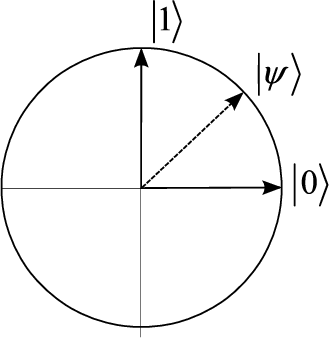
\includegraphics[scale=.3]{qubit_vector}
\end{figure}

Podemos determinar el estado de un bit clásico a la hora de examinarlo, pero en el caso del qubit, no podemos determinar el estado cuántico de un qubit en superposición, es decir, no podemos hallar el valor de $\alpha$ y $\beta$. Lo que sí podemos hacer es \textbf{medir} el qubit, determinar si colapsa en el estado $\ket{0}$ con probabilidad $|\alpha|^2$ ó en el estado $\ket{1}$ con probabilidad $|\beta|^2$. En otra palabras, el proceso de medir un qubit, nos devuelve como salida un estado clásico al que colapsa y deja de estar en superposición de varios estados de manera simultanea.

Veamos ahora otra representación geométrica del qubit que puede resultar útil. Consideramos un qubit en estado de superposición.
\begin{equation}
\ket{\psi} = c_0\ket{0} + c_1\ket{1} 
\end{equation}
con $\|c_0|^2 + |c_1|^2 = 1$. Reescribimos la expresión en coordenadas en forma exponencial de un número complejo,
\begin{equation}
\ket{\psi} = r_0 e^{i\varphi_0}\ket{0} + r_1 e^{i\varphi_1}\ket{1}
\end{equation}
Lo multiplicamos por un escalar de módulo 1, así no alteramos su estado cuántico,
\begin{equation}
e^{-i\varphi_0}\ket{\psi} = e^{-i\varphi_0}(r_0 e^{i\varphi_0}\ket{0} + r_1 e^{i\varphi_1}\ket{1}) = 
r_0\ket{0} + r_1 e^{i(\varphi_1 - \varphi_0)}\ket{1}
\end{equation}
Tomando ahora coordenadas polares $r_0 = \cos(\theta)$, $r_1 = \sin(\theta)$ y el cambio de variables $\varphi = \varphi_1 - \varphi_0$, resulta en la siguiente expresión,
\begin{equation}
\ket{\psi} = \cos(\theta)\ket{0} + e^{i\varphi}\sin(\theta)\ket{1}
\end{equation}
Considerando $\theta$ y $\varphi$ como coordenadas de un punto en una esfera tridimensional, podemos ver el estado del qubit como un punto en la superficie de dicha esfera, siendo los polos los estados $\ket{0}$ y $\ket{1}$. Esta esfera recibe el nombre de \textbf{esfera de Bloch} y veremos en poco que con ella podemos representar operaciones de qubits como rotaciones de la esfera.

\begin{figure}[h]
	\centering
	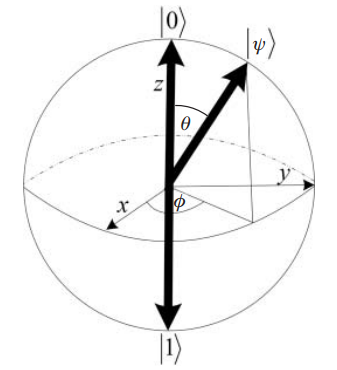
\includegraphics[scale=.3]{esfera_bloch}
	\caption{Esfera de Bloch.}
\end{figure}


\subsection{Sistema de Varios Qubits}

Tomamos interés en un sistema de un número mayor de qubits, que enlazaremos a través del producto tensorial de los espacios vectoriales. Por tanto un elemento de él estará representado por un vector de $\mathbb{C}^2 \otimes \mathbb{C}^2 \otimes \ldots \otimes \mathbb{C}^2$ que denotaremos como $(\mathbb{C}^2)^{\otimes n}$ donde $n$ es el número de qubits del sistema y cuya dimensión como espacio vectorial es $2^n$

Por ejemplo, si queremos un sistema de 2 qubits en comparación a los estados clásicos de un bit tendríamos 00, 01, 10 y 11, por tanto nuestro sistema de 2 qubits tendría los estados $\ket{00}$, $\ket{01}$, $\ket{10}$ y $\ket{11}$ que se corresponden con el producto tensorial del estado de los dos qubits $\ket{x}\otimes\ket{y}$ con $x$, $y\in \lbrace 0, 1\rbrace$.
Vamos a trabajar más cómodamente con coordenadas del vector en su expresión matricial, consideramos primero,
\begin{equation}
\ket{0} = \begin{bmatrix}
	1 \\ 0
\end{bmatrix}, \ 
\ket{1} = \begin{bmatrix}
	0 \\ 1
\end{bmatrix}
\end{equation}
Como hemos visto en la sección anterior, aplicaremos el producto de  Kroner para obtener las expresiones matriciales de $\ket{00}$, $\ket{01}$, $\ket{10}$ y $\ket{11}$,
\begin{equation}
\ket{00} =
\begin{bmatrix}
	1 \\ 0 \\ 0 \\ 0
\end{bmatrix}, \ 
\ket{01} =
\begin{bmatrix}
	0 \\ 1 \\ 0 \\ 0
\end{bmatrix}, \ 
\ket{10} =
\begin{bmatrix}
	0 \\ 0 \\ 1 \\ 0
\end{bmatrix}, \ 
\ket{11} =
\begin{bmatrix}
	0 \\ 0 \\ 0 \\ 1
\end{bmatrix}
\end{equation}
Observamos que forman una base ortonormal de un espacio vectorial de dimensión $2^2 = 4$ y que además cada coordenada corresponde a un estado clásico del qubit:
\begin{equation}
\ket{01} =
\begin{matrix}
	\textbf{00} \\ \textbf{01} \\ \textbf{10} \\ \textbf{11}
\end{matrix}
\begin{bmatrix}
	0 \\ 1 \\ 0 \\ 0
\end{bmatrix}
\end{equation}
Por tanto, si tomamos un sistema de dos qubits arbitrario en superposición,
\begin{equation}
\ket{\psi} = c_0 \ket{00} + c_1 \ket{01} + c_2 \ket{10} + c_3 \ket{11}
\end{equation}
su representación matricial sería:
\begin{equation}
\ket{\psi} =
\begin{matrix}
	\textbf{00} \\ \textbf{01} \\ \textbf{10} \\ \textbf{11}
\end{matrix}
\begin{bmatrix}
	c_0 \\ c_1 \\ c_2 \\ c_3
\end{bmatrix}
\end{equation}
Trabajaremos a partir de ahora con la notación del sistema de varios qubits como $\ket{xy}$, $\ket{x\otimes y}$, ó $\ket{x}\otimes\ket{y}$ y los trataremos de manera indiferente según convenga.

Podemos medir únicamente un subconjunto de qubits del sistema total siendo la probabilidad de obtener el qubit en un estado concreto la suma de las probabilidades del estado del sistema con el qubit correspondiente en el estado en concreto. Por ejemplo si tomamos el sistema de dos qubits anterior, la probabilidad de que el primer qubit esté en el estado $\ket{0}$ será $|c_0|^2 + |c_1|^2$ que son las probabilidades de que el sistema esté en el estado $\ket{00}$ ó $\ket{01}$. Hacemos notar que tras medirlo, el sistema quedará en el estado
\begin{equation}
\ket{\psi'} = \frac{c_0\ket{00} + c_1\ket{01}}{\sqrt{|c_0|^2 + |c_1|^2}}
\end{equation}
ya que hemos determinado el estado del primer qubit haciéndolo colapsar a un estado clásico a la hora de medirlo. Además, el denominador $\sqrt{|c_0|^2 + |c_1|^2}$ se debe por normalizar el vector que representa el estado del sistema. Recordemos que esto era una condición necesaria que tenemos que pedir.
Un ejemplo importante de un sistema de dos qubits es el \textbf{estado de Bell} ó \textbf{par ERP},
\begin{equation}
\frac{\ket{00} + \ket{11}}{\sqrt{2}}
\end{equation}
que nos muestra una propiedad importante de los sistemas de varios qubits a la hora de hacer mediciones. Si medimos el primer qubit tendrá una probabilidad de $(\frac{1}{\sqrt{2}})^2 = \frac{1}{2}$ de estar en el estado $\ket{0}$ y una probabilidad de $\frac{1}{2}$ de estar en el estado $\ket{1}$. Esto dejará el sistema en el estado $\ket{\psi'} = \ket{00}$ ó $\ket{\psi'} = \ket{11}$. En cualquier caso tenemos que ambas situaciones, tras medir el primer qubit, si medimos el segundo este coincidirá con el primero. Es decir, que ambos qubits está relacionados(entagled).

Nos fijamos un momento en la dimensión del espacio vectorial que representa nuestro sistema. Supongamos que tenemos un número de un tamaño considerable de qubits, $n=500$. Si quisiéramos simular este sistema en un ordenador clásico realizando las operaciones matriciales necesarias en la computación, tendríamos que para un estado del sistema almacenar $2^{500}$ coordenadas complejas del vector además de trabajar con matrices de tamaño $2^{500}$. Esto claramente no es factible hoy en día resultando en una de los problemas en cuanto a la computación cuántica.

\subsection{Circuitos y Puertas Cuánticas}

Al igual que un circuito de un ordenador clásico consiste en cables y puertas lógicas que interaccionan con la información que es transportada por el cableado, un circuito cuántico consiste en cables que transportan información cuántica en forma de qubits que son manipulados a través de puertas cuánticas.

Consideremos primero la puerta clásica \textbf{NOT} que queremos que realice la operación de la tabla de verdad sobre un bit, es decir,
\begin{equation}
\begin{cases}
0 \rightarrow 1 \\
1 \rightarrow 0
\end{cases}
\end{equation}
intercambiando los estados 0 y 1. Queremos que nuestra puerta cuántica se comporte de la misma manera sobre qubits. Queremos que intercambie los estados $\ket{0}$ y $\ket{1}$ y además por ser puerta cuántica pediremos que sea lineal, es decir, si tenemos un un qubit arbitrario en estado de superposición
\begin{equation}
\alpha\ket{0} + \beta\ket{1}
\end{equation}
queremos que se aplique de forma lineal a cada uno de los términos de la suma,
\begin{equation}
\alpha\ket{1} + \beta\ket{0}.
\end{equation}
Igual que hemos asociado con vectores a los bits, y podemos operar con los vectores de forma matricial, las puertas lógicas están asociados a las matrices.
Por tanto si tomamos la matriz $\textrm{NOT} = \begin{bmatrix} 0 & 1 \\ 1 & 0 \end{bmatrix}$, esta matriz cumple que
\begin{equation}
\begin{bmatrix}
0 & 1 \\
1 & 0
\end{bmatrix}
\begin{bmatrix}
1 \\ 0
\end{bmatrix} =
\begin{bmatrix}
0 \\ 1
\end{bmatrix}
\textrm{ y }
\begin{bmatrix}
0 & 1 \\
1 & 0
\end{bmatrix}
\begin{bmatrix}
0 \\ 1
\end{bmatrix} =
\begin{bmatrix}
1 \\ 0
\end{bmatrix}
\end{equation}
tomando el vector correspondiente al estado cuántico $\ket{0}$ y $\ket{1}$ y los intercambia:
\begin{equation}
\textrm{NOT} \ket{0} = \ket{1} \textrm{ y } \textrm{NOT}\ket{1} = \ket{0}
\end{equation}
Otra propiedad que les pediremos a las puertas cuánticas es que sean reversibles. Esto es que dados la salida y la operación aplicada seamos capaces de determinar la entrada del circuito. Representaremos las puertas cuánticas con matrices unitarias que son reversibles por su propia adjunta. Recordemos que esto es:
\begin{equation}
U * U^\dagger = U^\dagger * U = I_n
\end{equation}
Podemos poner de ejemplo, la operación AND, que toma dos bits y nos devuelve 1 si ambos inputs son 1. Esta operación no es reversible, ya que si conocemos solamente el output, no podemos determinar cuál ha sido el input de la operación. \\
De esta manera tenemos que, aparte de la propiedad de ser lineal que está implicada, cualquier matriz unitaria lleva asociada su puerta cuántica correspondiente, siendo el único requisito que pediremos.
Veamos otras puertas cuánticas de un qubits de importancia. Si consideramos las matrices de Pauli,
\begin{equation}
X = \begin{bmatrix}
	0 & 1 \\
	1 & 0
\end{bmatrix}, \ 
Y = \begin{bmatrix}
	0 & -i \\
	i & 0
\end{bmatrix}, \ 
Z = \begin{bmatrix}
	1 & 0 \\
	0 & -1
\end{bmatrix},
\end{equation}
tendremos que cada una de ellas tiene asociado una puerta cuántica correspondiente. De hecho, la matriz X corresponde con la puerta NOT. Podemos evaluar la matriz con los estados del qubit para determinar su comportamiento, pues por ejemplo si tomamos la matriz Z,
\begin{equation}
Z(\alpha\ket{0} + \beta\ket{1}) = 
\begin{bmatrix}
	1 & 0 \\
	0 & -1 
\end{bmatrix}
\begin{bmatrix}
	\alpha \\ \beta
\end{bmatrix} =
\begin{bmatrix}
	\alpha \\ -\beta
\end{bmatrix} =
\alpha\ket{0} - \beta\ket{1},
\end{equation}
que cambia el signo del coeficiente de $\ket{1}$.\\
Otra manera de visualizar estas puertas es como rotaciones de $180º$ sobre la esfera de Bloch en el eje correspondiente. \\
\begin{figure}[h]
	\centering
	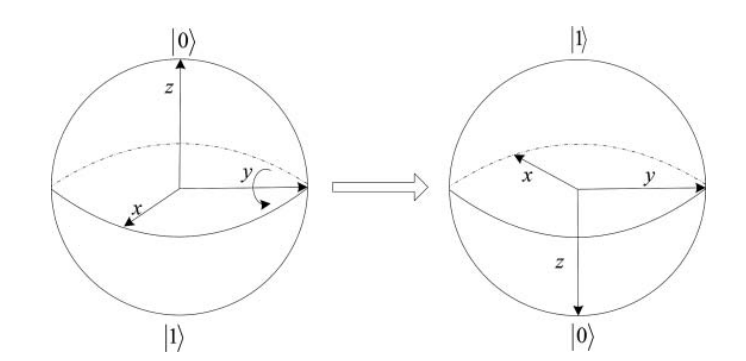
\includegraphics[scale=.65]{rotacion_bloch}
	\caption{Rotación sobre el eje Y en la esfera de Bloch.}
\end{figure}

Una puerta cuántica de mucha importancia es la puerta de Hadamard ya que nos permitirá poner qubit en una configuración en la que todos los estados son equiprobables. Esta puerta tiene por matriz:
\begin{equation}
\frac{1}{\sqrt{2}}
\begin{bmatrix}
1 & 1 \\
1 & -1
\end{bmatrix},
\end{equation}
que lleva
\begin{equation}
\begin{cases}
\ket{0} \rightarrow \frac{1}{\sqrt{2}}(\ket{0} + \ket{1}) \\
\ket{1} \rightarrow \frac{1}{\sqrt{2}}(\ket{0} - \ket{1})
\end{cases}
\end{equation}
Una propiedad que cumple $H^2 = I$ que se comprueba fácilmente. Esto nos permite posteriormente llevar estados $\frac{1}{\sqrt{2}}(\ket{0} + \ket{1})$ a $\ket{0}$, lo que usaremos posteriormente en los algoritmos.

Ya hemos mencionado que es posible visualizar las puertas cuánticas como rotaciones en la esfera de Bloch, por ejemplo si tomamos la expresión de un estado de un qubit en polares,
\begin{equation}
\ket{\psi} = \cos(\theta)\ket{0} + e^{i\varphi}\sin(\theta)\ket{1},
\end{equation}
y le aplicamos la siguiente matriz
\begin{equation}
R(\omega) = \begin{bmatrix}
	1 & 0 \\
	0 & e^\omega
\end{bmatrix} 
\end{equation}
obteniendo como resultado:
\begin{equation}
\ket{\psi'} = \cos(\theta)\ket{0} + e^\omega e^{i\varphi}\sin(\theta)\ket{1} = \cos(\theta)\ket{0} + e^{i\varphi + \omega}\sin(\theta)\ket{1}
\end{equation}
de esta manera hemos conseguido rotar la esfera alrededor del eje Z, por lo que no hemos variado lo que podemos considerar como latitud, sino hemos variado su longitud. Este tipo de operaciones se denominan \textbf{cambios de fase}, ya que sólo estamos alterando el valor del parámetro $e^{i\varphi}$, que denominaremos como \textbf{fase}. Observamos que esta alteración de la fase del estado del qubit no produce cambios en cuanto a la medición del mismo, ya que la probabilidad de que un qubit colapse en un estado clásico depende en este caso únicamente del parámetro $\theta$, su latitud en la esfera de Bloch, o también \textbf{amplitud}.

\begin{figure}[h]
	\centering
	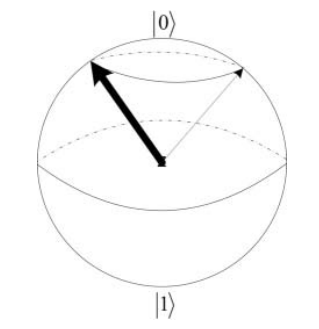
\includegraphics[scale=.65]{rotacion_fase}
\end{figure}
Otras rotaciones, por ejemplos si queremos rotar la espera un cierto ángulo $\omega$ respecto a un eje, tendría la siguiente expresión:
\begin{equation}
\begin{cases}
R_x(\omega) = \cos(\frac{\omega}{2})I -i\sin(\frac{\omega}{2})X =
\begin{bmatrix}
cos(\frac{\omega}{2}) & -i\sin(\frac{\omega}{2}) \\
-i\sin(\frac{\omega}{2}) & \cos(\frac{\omega}{2})
\end{bmatrix} \\
R_y(\omega) = \cos(\frac{\omega}{2})I -i\sin(\frac{\omega}{2})Y =
\begin{bmatrix}
	cos(\frac{\omega}{2}) & -\sin(\frac{\omega}{2}) \\
	\sin(\frac{\omega}{2}) & \cos(\frac{\omega}{2})
\end{bmatrix} \\
R_z(\omega) = \cos(\frac{\omega}{2})I -i\sin(\frac{\omega}{2})Z =
\begin{bmatrix}
	e^{-i\omega/2} & 0 \\
	0 & e^{i\omega/2}
\end{bmatrix}
\end{cases}
\end{equation}
También podemos realizar rotaciones respecto de un vector dado, consideramos $D = (D_x, D_y, D_z)$ un vector arbitrario de módulo 1, con las coordenadas correspondientes. La matriz de la rotación estará determinada por la siguiente expresión:
\begin{equation}
R_D(\omega) = \cos(\frac{\omega}{2})I -i\sin(\frac{\omega}{2})(D_x X + D_y Y + D_z Z)
\end{equation}
Veamos ahora, puertas cuánticas que involucren más de un qubit, que a pesar de que no podremos representarlos ya en la esfera de Bloch, podemos seguir considerando su representación matricial.

Una de las puertas más importantes es la puerta \textbf{NOT controlada} o \textbf{CNOT}. Esta puerta tomará dos entradas y dará dos salidas. La primera entrada la llamaremos bit de control, es decir, controlará el bit de salida. Representaremos la puerta en la siguiente ilustración de un circuito cuántico, donde cada recta horizontal representa un cable que lleva el qubit siguiendo la lectura de izquierda a derecha.
\begin{figure}[h]
\centering
\scalebox{1.0}{
\Qcircuit @C=1.0em @R=0.8em @!R { \\
	 \lstick{\ket{x}} & \ctrl{1} & \qw & \rstick{\ket{x}}\\
	 \lstick{\ket{y}} & \targ & \qw  & \rstick{\ket{x\oplus y}}\\
\\ }}
\end{figure}
Si $\ket{x} = \ket{0}$, la salida del segundo bit $\ket{y}$ permanecerá igual. Si  $\ket{x} = \ket{1}$ entonces $\ket{y}$ se le aplicará la puerta NOT, es decir, será lo opuesto. Es decir, realiza la siguiente transformación
\begin{equation}
\begin{cases}
\ket{00} \rightarrow \ket{00} \\
\ket{01} \rightarrow \ket{01} \\
\ket{10} \rightarrow \ket{11} \\
\ket{11} \rightarrow \ket{10}
\end{cases}
\end{equation}
Esto se puede ver como que la puerta transforma un par de bits $\ket{x, y}$ en $\ket{x, x\oplus y}$, donde $\oplus$ es la operación binaria de OR excluyente, o también como la suma en módulo 2.
También podemos describir la puerta CNOT con su representación matricial, considerando como base del espacio vectorial $\lbrace \ket{00}, \ket{01}, \ket{10}, \ket{11} \rbrace$,
\begin{equation}
\textrm{CNOT} = \begin{bmatrix}
1 & 0 & 0 & 0 \\
0 & 1 & 0 & 0 \\
0 & 0 & 0 & 1 \\
0 & 0 & 1 & 0 
\end{bmatrix}
\end{equation}
Observamos que claramente esta puerta es unitaria pues el producto por su adjunta que es ella misma resulta en la matriz identidad, pues tenemos que se cumple que $CNOT^{\dagger} CNOT = I$.
Esto también se puede entender como que la puerta CNOT es reversible por ella misma:\\
\begin{figure}[h]
\centering
\scalebox{1.0}{
\Qcircuit @C=1.0em @R=0.8em @!R { \\
	\nghost{0} & \ket{x} & \ & \ & \ & \ & \ket{x} & \ & \ & \ & \ket{x}  \\
	\nghost{1} & \qw & \qw & \qw & \ctrl{2} & \qw & \qw & \qw & \ctrl{2} & \qw & \qw & \qw \\
	\nghost{2} & \ket{y} & \ & \ & \ & \ & \ket{x\oplus y} & \ & \ & \ & \ & \ & \ket{x\oplus(x\oplus y)}  \\
	\nghost{3} & \qw & \qw & \qw & \targ & \qw & \qw & \qw & \targ & \qw & \qw & \qw \\
\\ }}
\end{figure}

El estado de entrada es $\ket{x, y}$ que queda trasformado en $\ket{x, x\oplus y}$ y esta última en $\ket{x, x\oplus (x\oplus y)}$. Esto es $\ket{x, (x\oplus x) \oplus y} = \ket{x, 0\oplus y} = \ket{x, y}$, ya que $x\oplus x = 0$.

Otra puerta reversible de mucha importancia es la de \textbf{Toffoli},
que funciona de manera similar a la puerta NOT controlada. Trabaja con 3 bits de entrada y salida, en el que aplica la puerta NOT al último bit $\ket{z}$ si y solo si los dos anteriores tienen por estado 1, $\ket{x, y} = \ket{11}$. En otras palabras lleva el $\ket{x,y,z}$ a $\ket{x,y,z\oplus(x\wedge y)}$. \\
\begin{figure}[h]
\centering
\scalebox{1.0}{
\Qcircuit @C=1.0em @R=0.8em @!R { \\
	 \lstick{\ket{x}} & \ctrl{1} & \qw & \rstick{\ket{x}}\\
	 \lstick{\ket{y}} & \ctrl{1} & \qw & \rstick{\ket{y}}\\
	 \lstick{\ket{z}} & \targ & \qw  & \rstick{\ket{z\oplus(x\wedge y)}}\\
\\ }}
\end{figure}

Esta puerta tiene por matriz:
\begin{equation}
\begin{bmatrix}
1 & 0 & 0 & 0 & 0 & 0 & 0 & 0 \\
0 & 1 & 0 & 0 & 0 & 0 & 0 & 0 \\
0 & 0 & 1 & 0 & 0 & 0 & 0 & 0 \\
0 & 0 & 0 & 1 & 0 & 0 & 0 & 0 \\
0 & 0 & 0 & 0 & 1 & 0 & 0 & 0 \\
0 & 0 & 0 & 0 & 0 & 1 & 0 & 0 \\
0 & 0 & 0 & 0 & 0 & 0 & 0 & 1 \\
0 & 0 & 0 & 0 & 0 & 0 & 1 & 0
\end{bmatrix}
\end{equation}
Ya hemos visto varias puertas que son reversibles, ahora, llamaremos puertas cuánticas a aquellas aplicaciones que actúan sobre qubits, como vectores de un espacio vectorial complejo y tendrá como representación matricial, matrices unitarias.

Una excepción de las puertas cuánticas sería la operación de medir un qubit, que se suelen realizar al final del circuito y que no son reversibles. Representaremos estas de la siguiente manera en el circuito, donde la doble recta horizontal, representa un cable que lleva información clásica, un bit.
\begin{figure}[h]
\centering
\scalebox{1.0}{
\Qcircuit @C=1.0em @R=0.8em @!R { \\
	 \nghost{cw} & \lstick{\ket{\psi}} & \qw & \meter & \cw & \cw\\
\\ }}
\end{figure}

Hemos visto varios ejemplos de circuitos cuánticos con las puertas cuánticas. Vamos a centrarnos en construir circuitos más complejos combinando las puertas. Podemos tanto concatenar las puertas, realizando una operación tras otra, y operar de manera paralela con ellas, de manera simultanea a un subconjunto del sistema de qubits. Hacemos notar varias restricciones respecto al mundo clásico y es que no permitiremos bucles en los circuitos, de manera que cada circuito funcione de izquierda a derecha y sea acíclico. Además no permitiremos tanto combinar dos cableado en uno, como dividir uno en dos. Veremos en un ejemplo próximo que de hecho no podemos copiar el estado de un qubit a otro.

En cuanto a concatenar las puertas en un circuito, simplemente realizaremos una operación tras otra, de manera ordenada. Si queremos tratar la operación como una matriz, esta se representará por productos de matrices de manera natural. Por ejemplo si queremos aplicar dos veces la puerta CNOT como hemos hecho antes,
\begin{equation}
\begin{bmatrix}
1 & 0 & 0 & 0 \\
0 & 1 & 0 & 0 \\
0 & 0 & 0 & 1 \\
0 & 0 & 1 & 0 
\end{bmatrix}
\begin{bmatrix}
1 & 0 & 0 & 0 \\
0 & 1 & 0 & 0 \\
0 & 0 & 0 & 1 \\
0 & 0 & 1 & 0 
\end{bmatrix} = 
\begin{bmatrix}
1 & 0 & 0 & 0 \\
0 & 1 & 0 & 0 \\
0 & 0 & 1 & 0 \\
0 & 0 & 0 & 1 
\end{bmatrix}
\end{equation}
resultando lo que esperábamos, ya que la puerta CNOT es reversible por sí misma, resultando que la concatenación de ella con sigo misma es la identidad.

También podemos realizar operaciones de manera paralela a distintos bits a través de productos tensoriales entre las matrices, siempre cuidando el tamaño de las matrices. Por ejemplo, si queremos aplicar la puerta de Hadamard $H$ a ambos qubits de un sistema de dos qubits, el resultado final será igual que aplicar $(H\otimes H)$ como una puerta al sistema,
\begin{figure}[h]
\centering
\scalebox{1.0}{
\Qcircuit @C=1.0em @R=0.8em @!R { \\
	 \lstick{\ket{x}} & \gate{\mathrm{H}} & \qw \\
	 \lstick{\ket{y}} & \gate{\mathrm{H}} & \qw \\
\\ }}
\end{figure}
Recordemos la propiedad del producto tensorial sobre las aplicaciones con la expresión \ref{prtensorial_aplineal}, de esta manera tenemos que,
\begin{equation} \label{matriz_tensorial}
(H\ket{x})\otimes(H\ket{y}) = (H\otimes H)\ket{x\otimes y}
\end{equation}
Vamos a ver un ejemplo más de circuito en el que concatenemos la puerta CNOT con la puerta de Hadamard. Consideramos entonces el circuito:
\begin{figure}[h]
\centering
\scalebox{1.0}{
\Qcircuit @C=1.0em @R=0.2em @!R { \\
	 	\lstick{\ket{x}} & \gate{\mathrm{H}} & \ctrl{1} & \qw & \qw\\
	 	\lstick{\ket{y}} & \qw & \targ & \qw & \qw &\ustick{\ket{\psi'}}\\
\\ }}
\end{figure}\\
Supongamos entonces que comenzaremos con el estado $\ket{00}$, para los otros casos el procedimiento es análogo. Entonces tendríamos que operar la siguiente expresión:
\begin{equation}
\ket{\psi'} = \textrm{CNOT}\cdot(H\otimes I)(\ket{x\otimes y})
\end{equation}
Hacemos notar que a pesar de que no le aplicamos ninguna puerta de manera simultanea a $\ket{y}$ para poder hacer el producto de matrices adecuadamente, es necesario aplicar el producto tensorial a la puerta de Hadamard con la identidad, que no altera el estado de $\ket{y}$.\\
Resolvamos entonces la expresión, con el estado $\ket{00}$ en concreto. Aplicando la propiedad de la expresión \ref{matriz_tensorial} , tenemos que:
\begin{equation}
\ket{\psi'} = \textrm{CNOT}\cdot(H\otimes I)(\ket{00}) = \textrm{CNOT}((H\ket{0}) \otimes (I\ket{0})) = \textrm{CNOT}(\frac{\ket{0}+\ket{1}}{\sqrt{2}}\otimes\ket{0})
\end{equation}
Reordenando la expresión con las propiedades del producto escalar tenemos que:
\begin{equation}
\ket{\psi'} = \textrm{CNOT}(\frac{1}{\sqrt{2}}(\ket{00} + \ket{10}))
\end{equation}
y finamente, aplicando la linealidad de CNOT:
\begin{equation}
\ket{\psi'} = \frac{1}{\sqrt{2}}(\textrm{CNOT}\ket{00} + \textrm{CNOT}\ket{10}) = \frac{1}{\sqrt{2}}(\ket{00} + \ket{11})
\end{equation}
Si recordamos de la sección anterior, hemos producido con este circuito empezando en el estado $\ket{00}$ al estado de Bell que hemos visto.\\
Este desarrollo de naturaleza algebraica que hemos hecho, tiene su equivalente en operaciones matriciales, pues podríamos haber hecho el producto de las matrices:
\begin{equation}
\textrm{CNOT}\cdot(H\otimes I) = \begin{bmatrix}
1 & 0 & 0 & 0 \\
0 & 1 & 0 & 0 \\
0 & 0 & 0 & 1 \\
0 & 0 & 1 & 0 
\end{bmatrix} \cdot \left( \frac{1}{\sqrt{2}}
\begin{bmatrix}
1 & 1 \\
1 & -1 
\end{bmatrix} \otimes
\begin{bmatrix}
1 & 0 \\
0 & 1 
\end{bmatrix}\right)
\end{equation}
Si operamos, obtendremos la siguiente matriz:
\begin{equation}
\frac{1}{\sqrt{2}}
\begin{bmatrix}
1 & 0 & 0 & 0 \\
0 & 1 & 0 & 0 \\
0 & 0 & 0 & 1 \\
0 & 0 & 1 & 0 
\end{bmatrix}
\begin{bmatrix}
1 & 0 & 1 & 0 \\
0 & 1 & 0 & 1 \\
1 & 0 & -1 & 0 \\
0 & 1 & 0 & -1 
\end{bmatrix} =
\frac{1}{\sqrt{2}}
\begin{bmatrix}
1 & 0 & 1 & 0 \\
0 & 1 & 0 & 1 \\
0 & 1 & 0 & -1 \\
1 & 0 & -1 & 0
\end{bmatrix}
\end{equation}
Por tanto si operamos con $\ket{00}$, tendremos:
\begin{equation}
\frac{1}{\sqrt{2}}
\begin{bmatrix}
1 & 0 & 1 & 0 \\
0 & 1 & 0 & 1 \\
0 & 1 & 0 & -1 \\
1 & 0 & -1 & 0
\end{bmatrix}
\begin{bmatrix}
1 \\ 0 \\ 0 \\ 0
\end{bmatrix} = 
\frac{1}{\sqrt{2}}
\begin{bmatrix}
1 \\ 0 \\ 0 \\ 1
\end{bmatrix}
\end{equation}
que es la expresión matricial del estado de Bell
\begin{equation}
\frac{\ket{00} + \ket{11}}{\sqrt{2}}
\end{equation}
\newpage

\section{Algoritmos Cuánticos}

En general, los algoritmos cuánticos siguen un esquema común entre ellos. Estos consistirán en:
\begin{itemize}
\item Comenzaremos con una serie de qubits en su estado clásico, es decir, $\ket{0}$ ó $\ket{1}$
\item Luego, serán puestos en superposición de varios estados.
\item Se le aplicarán una serie de operaciones unitarias a través de puertas cuánticas.
\item Y finalmente se medirán los qubits correspondientes y según el algoritmo, se repetirá este proceso varias veces y se compararán los resultados.

\end{itemize}

\subsection{Algoritmo de Teletransportación}
Empezaremos viendo un algoritmo sencillo que lo único que hará será teletransportar o mover un qubit en un estado arbitrario $\ket{\varphi}$ de un sitio a otro. Esta operación nos presenta los problemas más típicos del mundo cuántico, y es que no conocemos el estado $\ket{\varphi}$ en el que se encuentra el qubit, es decir, los valores de $\alpha$ y $\beta$ de $\ket{\varphi} = \alpha\ket{0} + \beta\ket{1}$. Además de que no podemos determinar sus valores con sólo una copia del qubit, y que sólo sabemos enviar información de manera clásica en forma de bits.\\

El algoritmo toma ventaja del enlazamiento entre qubits para superar los problemas. Consideramos un transmisor y un receptor, además de un par de qubits que se encuentra en el estado de Bell. Nuestro transmisor tiene el control de uno de los qubits, mientras que el receptor tiene el control del otro. El algoritmo consistirá entonces en el transmisor interactua con el qubit $\ket{\varphi}$ y su correspondiente qubit del par en estado de Bell, seguido de tomar mediciones de los dos qubits y enviar la información de los bits resultantes al receptor. Este último aplicará ciertas operaciones dependiendo de la información recibida a su qubit del par en estado de Bell, resultado en el qubit $\ket{\varphi}$.\\
Veamos esto en el circuito y revisemos las cuentas paso a paso. Consideramos el estado inicial de entrada $\ket{\varphi_0} = \ket{\varphi}\ket{\beta_{00}}$ que es un sistema de tres qubits formados por el qubit $\ket{\varphi}$ y un par de qubits en estado de Bell.

\begin{figure}[h]
\centering
\scalebox{1.5}{
\Qcircuit @C=1.0em @R=0.2em @!R { \\
	 	\rstick{\ket{\varphi}} & \nghost{} & \ctrl{1} & \gate{\mathrm{H}} & \meter & \cw & \controlo \cw_(0.4){\mathrm{M_1}} \cwx[2] \\
	 	\dstick{\ket{\beta_{00}}} & \nghost{} & \targ & \qw & \meter & \controlo \cw_(0.4){\mathrm{M_2}} \cwx[1]  \\
	 	\nghost{} & \nghost{} & \qw^(0.5){\ket{\varphi_0}} & \qw^(0.5){\ket{\varphi_1}} & \qw^(0.5){\ket{\varphi_2}} & \gate{\mathrm{Z^{M_2}}} & \gate{\mathrm{X^{M_1}}} & \qw &\rstick{\ket{\varphi}}\\}}
\end{figure}\ \linebreak
Ponemos el estado inicial en la expresión que nos conviene usando la propiedad distributiva respecto de la suma.
\begin{equation}
\begin{split}
\ket{\varphi_0} & =
 \ket{\varphi}\ket{\beta_{00}} =
\left[\alpha\ket{0} + \beta\ket{1}\right] \otimes \left[ \frac{\ket{00} + \ket{11}}{\sqrt{2}} \right] \\
& =
\frac{1}{\sqrt{2}} \left[ \alpha\ket{0}(\ket{00}+\ket{11}) + \beta\ket{1}(\ket{00}+\ket{11}) \right]
\end{split}
\end{equation}
Aplicamos la puerta CNOT a los dos primeros qubits, recordemos que la puerta CNOT cambia el estado del segundo qubit si el primero es un $1$, mientras que si el primer qubit es un $0$ dejará igual el sgundo qubit. Aprovechando entonces la linealidad de CNOT, tenemos por resultado
\begin{equation}
\ket{\varphi_1} = 
\frac{1}{\sqrt{2}} \left[ \alpha\ket{0}(\ket{00}+\ket{11}) + \beta\ket{1}(\ket{10}+\ket{01}) \right]
\end{equation}
Aplicamos entonces la puerta de Hadamard en el primer qubit, obteniendo
\begin{equation}
\ket{\varphi_2} = 
\frac{1}{\sqrt{2}} \left[ \alpha \left( \frac{\ket{0}+\ket{1}}{\sqrt{2}} \right) (\ket{00}+\ket{11}) + \beta\left( \frac{\ket{0}-\ket{1}}{\sqrt{2}} \right)(\ket{10}+\ket{01}) \right]
\end{equation}
Reordenamos la expresión
\begin{equation}
\begin{split}
\ket{\varphi_2} = 
\frac{1}{2} \left[ \alpha\left(\ket{000} + \ket{011} + \ket{100} + \ket{111}\right) + \beta\left(\ket{010} + \ket{001} - \ket{110} - \ket{101}\right) \right] = 
\\
\frac{1}{2} \left[ \ket{00}(\alpha\ket{0}+\beta\ket{1}) + \ket{01}(\alpha\ket{1}+\beta\ket{0}) + \ket{10}(\alpha\ket{0}-\beta\ket{1} + \ket{11}(\alpha\ket{1}-\beta\ket{0})) \right]
\end{split}
\end{equation}
Realizamos entonces la medición de los dos primeros qubits, que por estar enlazados los qubits, el resultado también determinará el estado del tercer qubit.
\begin{equation}
\begin{array}{l}
00 \longrightarrow \alpha\ket{0}+\beta\ket{1} \\
01 \longrightarrow \alpha\ket{1}+\beta\ket{0} \\
10 \longrightarrow \alpha\ket{0}-\beta\ket{1} \\
11 \longrightarrow \alpha\ket{1}-\beta\ket{0}
\end{array}
\end{equation}
Quedará finalmente realizar la transformación correspondiente al tercer qubit. Si el resultado de la medición es $00$ entonces no es necesario realizar ningún cambio pues tenemos que el estado del tercer qubit es $\alpha\ket{0}+\beta\ket{1} = \ket{\varphi}$. Si es $01$ tendremos que aplicar la puerta $X$ para transformar el $1$ en $0$ y el $0$ en $1$. Si es $10$ aplicaremos entonces la puerta $Z$ que cambia el signo de la segunda coordenada, el coeficiente de $\ket{1}$. Y finalmente, en el caso de $11$ aplicaremos primero la puerta $X$, seguido de la puerta $Z$.
Esto sería equivalente a aplicar la transformación $Z^{M_1} X^{M_2}$ con $M_1$ y $M_2$ el valor de los dos primeros qubits, recuperando entonces el estado $\ket{\varphi}$ en el qubit que controla el receptor.\\

Hacemos notar que hemos llevado el estado $\ket{\varphi}$ de un qubit a otro, pero no lo hemos copiado, pues el estado del primer qubit ha sido sobreescrito con las operaciones realizadas.
Como hemos mencionado antes, el proceso de copiar el estado de un qubit a otro no es posible. Podemos ver esto en que entra en contradicción con la propiedad lineal de las aplicaciones.\\ Suponemos $C$ una aplicación correspondiente a la operación cuántica de copiar el estado de un qubit a otro. La hacemos actuar sobre un par de qubits resultando en
\begin{equation}
C\left(\frac{\ket{x}+\ket{y}}{\sqrt{2}} \otimes \ket{0}\right) = 
\left(\frac{\ket{x}+\ket{y}}{\sqrt{2}} \otimes \frac{\ket{x}+\ket{y}}{\sqrt{2}}\right)
\end{equation}
Sin embargo, si aplicamos la propiedad lineal de $C$, tenemos que
\begin{equation}
\begin{split}
C\left(\frac{\ket{x}+\ket{y}}{\sqrt{2}} \otimes \ket{0}\right) 
&=
\frac{1}{\sqrt{2}}C\left((\ket{x}+\ket{y}) \otimes \ket{0}\right)
=
\frac{1}{\sqrt{2}} C(\ket{x}\otimes\ket{0} + \ket{y}\otimes\ket{0})
\\&=
\frac{1}{\sqrt{2}} C(\ket{x}\otimes\ket{0}) + C(\ket{y}\otimes\ket{0})
=
\frac{1}{\sqrt{2}} (\ket{x}\otimes\ket{x}) + (\ket{y}\otimes\ket{y})
\\&=
\frac{(\ket{x}\otimes\ket{x}) + (\ket{y}\otimes\ket{y})}{\sqrt{2}}
\end{split}
\end{equation}
Que claramente llegamos a resultados distintos, concluyendo en que hemos encontrado una contradicción. Por tanto la aplicación $C$ no es lineal y no se puede copiar estados de qubits.

\subsection{Algoritmo de Deutsch}

Veamos ahora un algoritmo simple que llamaremos como el algoritmo de Deutsch. Este algoritmo tratará de ver si se cumple cierta propiedad para una función $f:\{0, 1\} \rightarrow \{0, 1\}$, concretamente si es balanceada o constante.

\begin{deff}
Diremos que la función $f:\{0, 1\} \rightarrow \{0, 1\}$ es balanceada si $f(0) \neq f(1)$, y diremos que es constante si $f(0) = f(1)$.
\end{deff}
El algoritmo consistirá en tomar una función $f:\{0, 1\} \rightarrow \{0, 1\}$, que desconocemos su definición y sólo podremos evaluarla obteniendo su imagen con el objetivo de determinar si la función es balanceada o constante.\\
En un algoritmo clásico podríamos siempre evaluar la función en todos sus valores para determinar si es balanceada o constate. Esto nos llevaría un total de dos evaluaciones de la función. Veamos si el algoritmo cuántico puede mejorar esto ya que nos permite evaluar de manera simultanea sobre todos los valores posibles.\\
Para ello tomaremos una puerta cuántica que evaluará la función y observamos que esta tiene que ser reversible. Consideraremos la siguiente operación unitaria $U_f$. A esta función a veces nos referiremos como oráculo, ya que nos evaluará la función indicando la imagen sin que nosotros sepamos la definición de la función. Recordemos también está representado por una matriz unitaria.
\begin{figure}[h]
\centering
\scalebox{1.5}{
\Qcircuit @C=1.0em @R=0.8em @!R { \\
	 \lstick{\ket{x}} & \multigate{1}{\hspace{0.2cm}\mathrm{U_f}\hspace{0.2cm}} & \qw & \rstick{\ket{x}} \\
	 \lstick{\ket{y}} & \nghost{\hspace{0.2cm}\mathrm{U_f}\hspace{0.2cm}} \qw & \qw &  \rstick{\ket{y\oplus f(x)}}\\
\\ }}
\end{figure}\linebreak
En la primera entrada $\ket{x}$ será lo que queremos evaluar, y en la segunda entrada $\ket{y}$ actuará como un qubit de control. Tras el cuál, en la primera salida $\ket{x}$ permanecerá igual y en la segunda salida tendremos $\ket{y\oplus f(x)}$.\\
Observamos que esta puerta cuántica es reversible pues:

\begin{figure}[h]
\centering
\scalebox{1.5}{
\Qcircuit @C=1.0em @R=0.8em @!R {
	 \nghost{\ket{x}} & \qw_(0.0){\ket{x}} & \multigate{1}{\hspace{0.2cm}\mathrm{U_f}\hspace{0.2cm}} & \qw_(-0.4){\ket{x}} & \qw & \qw & \multigate{1}{\hspace{0.2cm}\mathrm{U_f}\hspace{0.2cm}} & \qw & \qw_(1.0){\ket{x}}  \\
	 \nghost{\ket{y}} & \qw_(0.0){\ket{y}} & \nghost{\hspace{0.2cm}\mathrm{U_f}\hspace{0.2cm}} \qw & \qw & \qw_(0.0){\ket{y\oplus f(x)}} & \qw & \nghost{\hspace{0.2cm}\mathrm{U_f}\hspace{0.2cm}} \qw & \qw_(-1.2){\ket{(y\oplus f(x))\oplus f(x)}} & \qw \\}}
\end{figure}\ \linebreak
El estado $\ket{x, y}$ queda trasformado en $\ket{x, y\oplus f(x)}$ y posteriormente en \\
$\ket{x, (y\oplus f(x))\oplus f(x)} = \ket{x, y\oplus (f(x)\oplus f(x))} = \ket{x, y\oplus 0} = \ket{x, y}$, ya que $f(x)\oplus f(x) = 0$.\\
Una vez conseguido el oráculo que nos evaluará la función en los qubits, podemos construir el circuito del algoritmo que consistirá en lo siguiente:

\begin{figure}[h]
\centering
\scalebox{1.5}{
\Qcircuit @C=1.0em @R=0.8em @!R { \\
	 \nghost{\ket{x}} & \qw_(0.0){\ket{0}} & \gate{\mathrm{H}} & \qw & \multigate{1}{\hspace{0.2cm}\mathrm{U_f}\hspace{0.2cm}} & \qw & \gate{\mathrm{H}} & \qw & \meter \\
	 \nghost{\ket{y}} & \qw_(0.0){\ket{1}} & \gate{\mathrm{H}} & \qw^(0.0){\ket{\varphi_1}} & \nghost{\hspace{0.2cm}\mathrm{U_f}\hspace{0.2cm}} \qw & \qw^(0.0){\ket{\varphi_2}} & \qw & \qw^(0.0){\ket{\varphi_3}} & \qw \\}}
\end{figure}\ \linebreak
Esto en términos matriciales sería:
\begin{equation}
(H\oplus I) U_f (H\oplus H) \ket{0, 1} = 
(H\oplus I) U_f (H\oplus H)
\begin{bmatrix}
0 \\ 1 \\ 0 \\ 0
\end{bmatrix}
\end{equation}
Veamos en detalle el resultado al que se llega. Empezamos con el estado $\ket{\varphi_0} = \ket{0, 1}$ que pondremos en superposición con la puerta de Hadamard.
Hadamard transforma a $\ket{0}$ en $\frac{\ket{0} + \ket{1}}{\sqrt{2}}$ y $\ket{1}$ en $\frac{\ket{0} - \ket{1}}{\sqrt{2}}$, por tanto,
\begin{equation}
\ket{\varphi_1} = \left[ \frac{\ket{0} + \ket{1}}{\sqrt{2}} \right] \left[ \frac{\ket{0} - \ket{1}}{\sqrt{2}} \right] =
\frac{\ket{0,0} - \ket{0,1} + \ket{1,0} - \ket{1,1}}{2} = 
\begin{bmatrix}
+\frac{1}{2} \\ -\frac{1}{2} \\ +\frac{1}{2} \\ -\frac{1}{2}
\end{bmatrix}
\end{equation}
Ahora, aplicaremos el oráculo $U_f$ a la expresión $\frac{\ket{0,0} - \ket{0,1} + \ket{1,0} - \ket{1,1}}{2}$ y recordando que $U_f$ no deja de ser una aplicación lineal. Por tanto, tenemos que
\begin{equation}
\ket{\varphi_2} = U_f \frac{\ket{0,0} - \ket{0,1} + \ket{1,0} - \ket{1,1}}{2} = \frac{U_f\ket{0,0} - U_f\ket{0,1} + U_f\ket{1,0} - U_f\ket{1,1}}{2} 
\end{equation}
Recordemos que nuestro oráculo $U_f$ transforma $\ket{x,y}$ en $\ket{x,y\oplus f(x)}$, por lo que
\begin{equation}
\begin{split}
\ket{\varphi_2} =
\frac{\ket{0,0\oplus f(0)} - \ket{0,1\oplus f(0)} + \ket{1, 0\oplus f(1)} - \ket{1, 1\oplus f(1)}}{2} = \\
\frac{\ket{0,f(0)} - \ket{0,\overline{f(0)}} + \ket{1,f(1)} - \ket{1,\overline{f(1)}}}{2}
\end{split}
\end{equation}
donde $\overline{f(x)}$ es el opuesto de $f(x)$.\\
Hacemos ver que $\ket{x,y}$ no es más que una notación de $\ket{x}\otimes\ket{y}$, por tanto aplicando la propiedad distributiva del producto tensorial por la derecha tenemos
\begin{equation} \label{eq45}
\ket{\varphi_2} =
\frac{\ket{0} \otimes \left[ \ket{f(0)} - \ket{\overline{f(0)}} \right] + \ket{1} \otimes \left[ \ket{f(1)} - \ket{\overline{f(1)}} \right]}{2}
\end{equation}
Observemos en un momento la expresión $\ket{f(x)} -\ket{\overline{f(x)}}$ para $x \in \lbrace 0,1 \rbrace$ y discutimos su valor según el valor de $f(x)$.
\begin{equation} \label{eq413}
\ket{f(x)} - \ket{\overline{f(x)}} =
\begin{cases}
\ket{0} - \ket{1} \ \textrm{si} \ f(x) = 0 \\
\ket{1} - \ket{0} \ \textrm{si} \ f(x) = 1
\end{cases} =
\begin{cases}
\ket{0} - \ket{1} \ \textrm{si} \ f(x) = 0 \\
-(\ket{0} - \ket{1}) \ \textrm{si} \ f(x) = 1
\end{cases}
\end{equation}
que escribiremos como $(-1)^{f(x)}(\ket{0} - \ket{1})$.\\
Aplicando esto a la expresión \ref{eq45} tenemos que
\begin{equation}
\ket{\varphi_2} = 
\frac{(-1)^{f(0)} (\ket{0} \otimes \left[ \ket{0} - \ket{1} \right]) + (-1)^{f(1)} (\ket{1} \otimes \left[ \ket{0} - \ket{1} \right])}{2}
\end{equation}
Hacemos uso de la propiedad distributiva por la derecha y reordenamos los escalares para separar la expresión en producto escalar de dos términos
\begin{equation}
\ket{\varphi_2} =
\left[ \frac{(-1)^{f(0)} \ket{0} + (-1)^{f(1)} \ket{1}}{\sqrt{2}} \right]
\left[ \frac{\ket{0} - \ket{1}}{\sqrt{2}} \right]
\end{equation}
Discutamos el valor de la expresión $(-1)^{f(0)} \ket{0} + (-1)^{f(1)} \ket{1}$ según si $f(x)$ es constante o balanceada.
\begin{equation}
\ket{\varphi_2} = 
\begin{cases}
(\pm 1) \left[\frac{\ket{0}+\ket{1}}{2}\right] \left[\frac{\ket{0}-\ket{1}}{2}\right] & \textrm{si } f \textrm{ es constante,} \\
(\pm 1) \left[\frac{\ket{0}-\ket{1}}{2}\right] \left[\frac{\ket{0}-\ket{1}}{2}\right] & \textrm{si } f \textrm{ es balanceada.}
\end{cases}
\end{equation}
Teniendo en cuenta que Hadamard es su propia inversa, llevará $\frac{\ket{0}+\ket{1}}{2}$ a $\ket{0}$ y $\frac{\ket{0}-\ket{1}}{2}$ a $\ket{1}$.
\begin{equation}
\ket{\varphi_3} = 
\begin{cases}
(\pm 1) \ket{0} \left[\frac{\ket{0}-\ket{1}}{2}\right] & \textrm{si } f \textrm{ es constante,} \\
(\pm 1) \ket{1} \left[\frac{\ket{0}-\ket{1}}{2}\right] & \textrm{si } f \textrm{ es balanceada.}
\end{cases}
\end{equation}
Finalmente medimos el qubit superior para determinar si f es constante o balanceada, ya que si sale $\ket{0}$ será constante y si sale $\ket{1}$ será balanceada. Observamos que el signo no afecta a la proceso de medir, pues recordemos que la probabilidad de que sea un estado depende de la norma al cuadrado.\\
Observamos que hemos conseguido en una evaluación de la función determinar si la propiedad de ser balanceada o constante. Sin embargo hacemos notar que para determinar cuál de los cuatro posibles funciones es, necesitamos evaluar de nuevo la función con este algoritmo.

\newpage

\subsection{Algoritmo de Deutsch-Jozsa}
Veremos ahora el mismo problema pero generalizando la función. Consideramos ahora la función $f:\{0, 1\}^n \longrightarrow \{0, 1\}$ que lleva cadenas de $n$ $0$ y $1$ a un único $0$ ó $1$ como imagen.\\
\begin{deff}
Diremos entonces que $f:\{0, 1\}^n \longrightarrow \{0, 1\}$ es balanceada si exactamente la mitad de los elementos del dominio de la función tiene a $0$ por imagen, y la otra mitad a $1$. Diremos también que la función es constante si todos los elementos tiene como imagen el $0$ ó si todos los elementos tiene como imagen el $1$.
\end{deff}
El algoritmo de Deutsch-Jozsa resuelve el problema de dada una función $f:\{0, 1\}^n \longrightarrow \{0, 1\}$ con la que podemos evaluar pero no sabemos cómo está definido, suponiendo que la función sólo puede ser balanceada o constante, tenemos que determinar cuál de estas dos propiedades cumple.\\

Veamos primero como se podría resolver utilizando un método clásico. Se podría evaluar la función diferentes valores para poder determinar si es balanceada o constante. En el mejor de los casos, si tras dos evaluaciones se llega a dos imágenes distintas, podemos concluir que es balanceada pues está asegurado que cumpla una de las propiedades. En el peor de los casos se requiere evaluar la mitad de los elementos más uno, si todas las imágenes comprobadas son iguales se llega a que la función es constante, en otro caso será balanceada. Esto requiere en el pero de los casos $\frac{2^n}{2}+1$ evaluaciones de la función, veamos si con el algoritmo cuántico se puede mejorar.\\
\linebreak
El algoritmo consistirá como el anterior, pondremos los qubits en estado de superposición para poder evaluarlos de manera simultanea en el oráculo. Este tendrá la siguiente forma, que se podrá representar con una matriz unitaria.\\
\begin{figure}[h]
\centering
\scalebox{1.5}{
\Qcircuit @C=1.0em @R=0.8em @!R {
	 \lstick{\ket{\mathbf{x}}} & \qw & \lstick{/^{n}} \qw & \multigate{1}{\hspace{0.2cm}\mathrm{U_f}\hspace{0.2cm}} & \qw & \lstick{/^{n}} \qw & \rstick{\ket{\mathbf{x}}} \\
	 \lstick{\ket{y}} & \qw & \qw & \nghost{\hspace{0.2cm}\mathrm{U_f}\hspace{0.2cm}} \qw & \qw & \qw & \rstick{\ket{y\oplus f(\mathbf{x})}}
	 \\}}
\end{figure}\linebreak
donde \Qcircuit @C=1.0em @R=0.8em @!R {\nghost{} & \qw & \lstick{/^{n}} \qw & \nghost{}} indica que hay $n$ qubits y usaremos $\ket{\mathbf{x}} = \ket{x_0 x_1\dots x_{n-1}}$ para denotar la cadena binaria. En este caso, $\ket{\mathbf{x}}$ quedará igual tras el oráculo $U_f$, mientras que $\ket{y}$ será el qubit de control. Es fácil ver que, como en el algoritmo anterior, el oráculo $U_f$ es reversible por sí misma.\\

Una vez obtenido el oráculo, queremos poner en superposición los $n$ qubits. Para ello usaremos la matriz de Hadamard, concretamente el producto tensorial de $n$ matrices de Hadamard. Veamos primero qué forma tiene esta matriz. Recordemos que la matriz de Hadamard tiene esta forma:
\begin{equation}
H = \frac{1}{\sqrt{2}}
\begin{bmatrix}
1 & 1 \\
1 & -1
\end{bmatrix}
\end{equation}\linebreak
Observamos que el elemento de la fila $i$ columna $j$ se puede expresar como $H[i, j] = \frac{1}{\sqrt{2}}(-1)^{i\wedge j}$, con $i$ y $j$ expresado en binario y $\wedge$ es la operación AND. De esta manera, la matriz de queda escrito como:
\begin{equation}
H = \frac{1}{\sqrt{2}}
\begin{bmatrix}
(-1)^{0\wedge 0} & (-1)^{0\wedge 1} \\
(-1)^{1\wedge 0} & (-1)^{1\wedge 1}
\end{bmatrix}
\end{equation}
Calculemos ahora el producto tensorial de dos matrices de Hadamard, que lo podemos expresar en forma de potencias de matrices con el producto tensorial que denotaremos como
\begin{equation}
H^{\otimes 2} = H\otimes H =
\frac{1}{\sqrt{2}}
\begin{bmatrix}
(-1)^{0\wedge 0} & (-1)^{0\wedge 1} \\
(-1)^{1\wedge 0} & (-1)^{1\wedge 1}
\end{bmatrix}\otimes
\frac{1}{\sqrt{2}}
\begin{bmatrix}
(-1)^{0\wedge 0} & (-1)^{0\wedge 1} \\
(-1)^{1\wedge 0} & (-1)^{1\wedge 1}
\end{bmatrix}
\end{equation}
\newpage
\begin{equation}
H^{\otimes 2} =
\frac{1}{\sqrt{2}} \cdot \frac{1}{\sqrt{2}}
\begin{bmatrix}
(-1)^{0\wedge 0}\cdot(-1)^{0\wedge 0} & (-1)^{0\wedge 0}\cdot(-1)^{0\wedge 1} & (-1)^{0\wedge 1}\cdot(-1)^{0\wedge 0} & (-1)^{0\wedge 1}\cdot(-1)^{0\wedge 1} 
\\
(-1)^{0\wedge 0}\cdot(-1)^{1\wedge 0} & (-1)^{0\wedge 0}\cdot(-1)^{1\wedge 1} & (-1)^{0\wedge 1}\cdot(-1)^{1\wedge 0} & (-1)^{0\wedge 1}\cdot(-1)^{1\wedge 1} 
\\
(-1)^{1\wedge 0}\cdot(-1)^{0\wedge 0} & (-1)^{1\wedge 0}\cdot(-1)^{0\wedge 1} & (-1)^{1\wedge 1}\cdot(-1)^{0\wedge 0} & (-1)^{1\wedge 1}\cdot(-1)^{0\wedge 1} 
\\
(-1)^{1\wedge 0}\cdot(-1)^{1\wedge 0} & (-1)^{1\wedge 0}\cdot(-1)^{1\wedge 1} & (-1)^{1\wedge 1}\cdot(-1)^{1\wedge 0} & (-1)^{1\wedge 1}\cdot(-1)^{1\wedge 1}
\end{bmatrix}
\end{equation}
Teniendo en cuenta que estamos interesados sólo por el signo de $(-1)^x$ que depende de la paridad de $x$, podemos considerar el producto de $(-1)^x\cdot(-1)^y$ como $(-1)^{x\oplus y}$, donde $\oplus$ es la suma módulo $2$. Entonces, la matriz sería
\begin{equation}
\begin{split}
H^{\otimes 2} =
\frac{1}{2}
\begin{bmatrix}
(-1)^{0\wedge 0\oplus 0\wedge 0} & (-1)^{0\wedge 0\oplus 0\wedge 1} & (-1)^{0\wedge 1\oplus 0\wedge 0} & (-1)^{0\wedge 1\oplus 0\wedge 1} 
\\
(-1)^{0\wedge 0\oplus 1\wedge 0} & (-1)^{0\wedge 0\oplus 1\wedge 1} & (-1)^{0\wedge 1\oplus 1\wedge 0} & (-1)^{0\wedge 1\oplus 1\wedge 1} 
\\
(-1)^{1\wedge 0\oplus 0\wedge 0} & (-1)^{1\wedge 0\oplus 0\wedge 1} & (-1)^{1\wedge 1\oplus 0\wedge 0} & (-1)^{1\wedge 1\oplus 0\wedge 1} 
\\
(-1)^{1\wedge 0\oplus 1\wedge 0} & (-1)^{1\wedge 0\oplus 1\wedge 1} & (-1)^{1\wedge 1\oplus 1\wedge 0} & (-1)^{1\wedge 1\oplus 1\wedge 1}
\end{bmatrix}
\\=
\frac{1}{2}
\begin{bmatrix}
1 & 1 & 1 & 1 \\
1 & -1 & 1 & -1 \\
1 & 1 & -1 & -1 \\
1 & -1 & -1 & 1
\end{bmatrix}
\end{split}
\end{equation}
De esta manera si definimos la aplicación $\langle \ , \ \rangle : \{0, 1\}^n \times \{0, 1\}^n \longrightarrow \{0, 1\}$ de manera que dados dos cadenas binarias de longitud $n$, $\mathbf{x} = x_0 x_1\ldots x_{n-1}$ y $\mathbf{y} = y_0 y_1\ldots y_{n-1}$, se define
\begin{equation}
\begin{split}
\langle \mathbf{x}, \mathbf{y} \rangle &= \langle x_0 x_1\ldots x_{n-1}, y_0 y_1\ldots y_{n-1} \rangle \\&= (x_0 \wedge y_0) \oplus (x_1 \wedge y_1) \oplus \ldots \oplus (x_{n-1} \wedge y_{n-1})
\end{split}
\end{equation}
Observamos que esta aplicación es en realidad el producto escalar del espacio vectorial cuyo cuerpo es el espacio $\mathbb{Z}_2$. Por tanto, podemos expresar $H^{\otimes 2}$ como
\begin{equation}
\begin{bmatrix}
(-1)^{\langle 00, 00 \rangle} & (-1)^{\langle 00, 01 \rangle} & (-1)^{\langle 00, 10 \rangle} & (-1)^{\langle 00, 11 \rangle} 
\\
(-1)^{\langle 01, 00 \rangle} & (-1)^{\langle 01, 01 \rangle} & (-1)^{\langle 01, 10 \rangle} & (-1)^{\langle 01, 11 \rangle} 
\\
(-1)^{\langle 10, 00 \rangle} & (-1)^{\langle 10, 01 \rangle} & (-1)^{\langle 10, 10 \rangle} & (-1)^{\langle 10, 11 \rangle} 
\\
(-1)^{\langle 11, 00 \rangle} & (-1)^{\langle 11, 01 \rangle} & (-1)^{\langle 11, 10 \rangle} & (-1)^{\langle 11, 11 \rangle}
\end{bmatrix}
\end{equation}
Ahora, si queremos generalizarlo para $H^{\otimes n}$ tenemos que su elemento de la fija $i$ columna $j$ expresado los indices en binario, es
\begin{equation}
H^{\otimes n} = \frac{1}{\sqrt{2^n}}(-1)^{\langle i, j \rangle}
\end{equation}
Entonces, si consideramos un estado arbitrario $\ket{\mathbf{y}}$ que estará representado por un vector con un $1$ en la posición $\mathbf{y}$ y el resto $0$ y le aplicamos $H^{\otimes n}$, obtendremos la suma de los elementos de la columna $\mathbf{y}$ de la matriz, es decir,
\begin{equation} \label{gHadamard}
H^{\otimes n}\ket{\mathbf{y}} =
\frac{1}{\sqrt{2^n}}\sum_{\mathbf{x}\in \{ 0, 1\}^n} (-1)^{\langle \mathbf{x}, \mathbf{y} \rangle} \ket{\mathbf{x}}
\end{equation}
Así podremos poner nuestros qubits en un estado de superposición de todos los estados posibles. Por ejemplo podemos tomar el estado $\ket{\mathbf{0}}$ y al aplicarle $H^{\otimes n}$ esta será
\begin{equation} \label{eq427}
H^{\otimes n}\ket{\mathbf{0}} = 
\frac{1}{\sqrt{2^n}}\sum_{\mathbf{x}\in \{ 0, 1\}^n} (-1)^{\langle \mathbf{x}, \mathbf{0} \rangle} \ket{\mathbf{x}} =
\frac{1}{\sqrt{2^n}}\sum_{\mathbf{x}\in \{ 0, 1\}^n} \ket{\mathbf{x}}
\end{equation}
ya que $\langle \mathbf{x}, \mathbf{0} \rangle = 0$, para cualquier valor $\mathbf{x}$.

\newpage

Una vez aclarado esto, podemos proceder a ver el circuito del algoritmo. De manera similar al algoritmo anterior, comenzaremos con $\ket{\mathbf{0}} = \ket{00\ldots 0}$ siendo una cadena de $0$ como el estado de los primeros $n$ qubits, y $\ket{1}$ el qubit de control. Aplicaremos la puerta $H^{\otimes n}$ para poner los primeros $n$ qubits en superposición.

\begin{figure}[h]
\centering
\scalebox{1.5}{
\Qcircuit @C=1.0em @R=0.8em @!R { \\
	 \nghost{\ket{x}} & \rstick{/^{n}} \qw_(0.0){\ket{\mathbf{0}}} & \qw & \gate{\mathrm{H}^{\otimes n}} & \qw & \lstick{/^{n}} \qw & \multigate{1}{\hspace{0.3cm}\mathrm{U_f}\hspace{0.3cm}} & \qw & \lstick{/^{n}} \qw & \gate{\mathrm{H^{\otimes n}}} & \qw & \lstick{/^{n}} \qw & \meter \\
	 \nghost{\ket{y}} & \qw_(0.0){\ket{1}} & \qw^(0.0){\ket{\varphi_0}} & \gate{\mathrm{H}} & \qw^(0.0){\ket{\varphi_1}} & \qw & \nghost{\hspace{0.3cm}\mathrm{U_f}\hspace{0.3cm}} \qw & \qw^(0.0){\ket{\varphi_2}} & \qw & \qw & \qw^(0.0){\ket{\varphi_3}} & \qw & \qw \\}}
\end{figure}\ \linebreak
O en término de matrices, esto sería:
\begin{equation}
\left( H^{\otimes n} \otimes I \right) U_f \left( H^{\otimes n} \otimes H \right) \ket{\mathbf{0}, 1}
\end{equation}
Empezamos entonces con el estado $\ket{\varphi_0} = \ket{\mathbf{0}, 1}$ y le aplicamos la matriz de Hadamard, usando la expresión \ref{eq427} y reordenando por la propiedad distributiva
\begin{equation}
\begin{split}
\ket{\varphi_1} &= (H^{\otimes n}\otimes H)\ket{\mathbf{0}, 1} =
\left[H^{\otimes n}\ket{\mathbf{0}} \right] \otimes \left[ H\ket{1} \right] =
\left[ \frac{1}{\sqrt{2^n}} \sum_{\mathbf{x}\in\{ 0, 1\}^n} \ket{\mathbf{x}} \right] \left[ \frac{\ket{0}-\ket{1}}{\sqrt{2}} \right] \\&=
\frac{1}{\sqrt{2^n}} \sum_{\mathbf{x}\in\{ 0, 1\}^n} \left[ \frac{\ket{\mathbf{x}, 0}-\ket{\mathbf{x}, 1}}{\sqrt{2}} \right]
\end{split}
\end{equation}
Aplicamos $U_f$ recordando que es un aplicación lineal que lleva $\ket{\mathbf{x}, y}$ a $\ket{\mathbf{x}, y\oplus f(\mathbf{x})}$
\begin{equation}
\begin{split}
\ket{\varphi_2} &= U_f
\frac{1}{\sqrt{2^n}} \sum_{\mathbf{x}\in\{ 0, 1\}^n} \left[ \frac{\ket{\mathbf{x}, 0}-\ket{\mathbf{x}, 1}}{\sqrt{2}} \right]
= 
\frac{1}{\sqrt{2^n}} \sum_{\mathbf{x}\in\{ 0, 1\}^n} \left[ \frac{U_f\ket{\mathbf{x}, 0} - U_f\ket{\mathbf{x}, 1}}{\sqrt{2}} \right]
\\ &=
\frac{1}{\sqrt{2^n}} \sum_{\mathbf{x}\in\{ 0, 1\}^n} \left[ \frac{\ket{\mathbf{x}, 0\oplus f(\mathbf{x})} - \ket{\mathbf{x}, 1\oplus f(\mathbf{x})}}{\sqrt{2}} \right] =
\frac{1}{\sqrt{2^n}} \sum_{\mathbf{x}\in\{ 0, 1\}^n} \ket{\mathbf{x}} \left[ \frac{\ket{f(\mathbf{x})} - \ket{\overline{f(\mathbf{x})}}}{\sqrt{2}} \right]
\end{split}
\end{equation}
donde $\overline{f(\mathbf{x})}$ es el opuesto. Recordemos ahora de expresión \ref{eq413} que podemos poner $\ket{f(\mathbf{x})} - \ket{\overline{f(\mathbf{x})}}$ como $(-1)^{f(\mathbf{x})}(\ket{0} - \ket{1})$, por tanto sustituyendo en la expresión anterior obtenemos
\begin{equation} \label{eq431}
\ket{\varphi_2} =
\left[ \frac{1}{\sqrt{2^n}} \sum_{\mathbf{x}\in\{ 0, 1\}^n} (-1)^{f(\mathbf{x})} \ket{\mathbf{x}} \right] \left[ \frac{\ket{0} - \ket{1}}{\sqrt{2}} \right]
\end{equation}
Aplicando ahora la matriz $H^{\otimes n}$ a los primeros $n$ qubits, aprovechando la expresión \ref{gHadamard} y que es lineal tenemos que
\begin{equation}
\begin{split}
\ket{\varphi_3} &=
\left[H^{\otimes n}\frac{1}{\sqrt{2^n}} \sum_{\mathbf{x}\in\{ 0, 1\}^n} (-1)^{f(\mathbf{x})} \ket{\mathbf{x}} \right] \left[ \frac{\ket{0} - \ket{1}}{\sqrt{2}} \right] =
\left[\frac{1}{\sqrt{2^n}} \sum_{\mathbf{x}\in\{ 0, 1\}^n} (-1)^{f(\mathbf{x})} H^{\otimes n}\ket{\mathbf{x}} \right] \left[ \frac{\ket{0} - \ket{1}}{\sqrt{2}} \right]
\\&=
\left[\frac{1}{2^n} \sum_{\mathbf{x}\in\{ 0, 1\}^n} (-1)^{f(\mathbf{x})} \sum_{\mathbf{z}\in\{ 0, 1\}^n} (-1)^{\langle \mathbf{z}, \mathbf{x} \rangle} \ket{\mathbf{z}} \right] \left[ \frac{\ket{0} - \ket{1}}{\sqrt{2}} \right]
\end{split} 
\end{equation}
Ahora juntamos las dos potencias de $(-1)$ teniendo en cuenta que estamos interesados por la paridad del exponente, usamos $\oplus$ la suma módulo $2$.
\begin{equation}
\ket{\varphi_3} =
\left[\frac{ \sum_{\mathbf{x}\in\{ 0, 1\}^n} \sum_{\mathbf{z}\in\{ 0, 1\}^n} (-1)^{f(\mathbf{x}) \oplus \langle \mathbf{z}, \mathbf{x} \rangle} \ket{\mathbf{z}} } {2^n} \right] \left[ \frac{\ket{0} - \ket{1}}{\sqrt{2}} \right]
\end{equation}
\newpage
Finalmente nos queda medir los $n$ primeros qubits. Nos preguntamos cuál es la probabilidad de que esté en el estado $\ket{\mathbf{0}}$, fijando $\mathbf{z} = \mathbf{0}$. Por tanto, como $\langle \mathbf{z}, \mathbf{x} \rangle = \langle \mathbf{0}, \mathbf{x} \rangle = 0$ para todo $\mathbf{x}$, tenemos que la probabilidad es
\begin{equation}
\left\vert \frac{\sum_{\mathbf{x}\in\{ 0, 1\}^n} (-1)^{f(\mathbf{x})}}{2^n} \right\vert^2 
\end{equation}
Observamos que depende únicamente de $f(\mathbf{x})$ por lo que podemos discutir su valor según $f(\mathbf{x})$.\\
Si $f(\mathbf{x})$ es constantemente $0$ ó $1$ tenemos que la probabilidad de estar en el estado $\ket{\mathbf{0}}$ es
\begin{equation}
\left\vert \frac{\sum_{\mathbf{x}\in\{ 0, 1\}^n} (-1)^{f(\mathbf{x})}}{2^n} \right\vert^2  =
\left\vert \frac{\sum_{\mathbf{x}\in\{ 0, 1\}^n} (\pm 1)}{2^n} \right\vert^2 =
\left\vert \frac{\pm 2^n}{2^n} \right\vert^2 = 1
\end{equation}
Si $f(\mathbf{x})$ es balanceada, la mitad de los términos $(-1)^{f(\mathbf{x})}$ anulan a la otra mitad y se obtiene que la probabilidad es
\begin{equation}
\left\vert \frac{\sum_{\mathbf{x}\in\{ 0, 1\}^n} (-1)^{f(\mathbf{x})}}{2^n} \right\vert^2  =
\left\vert \frac{\sum_{\mathbf{x}\in\{ 0, 1\}^n} 0}{2^n} \right\vert^2 =
\left\vert \frac{0}{2^n} \right\vert^2 = 0
\end{equation}
Podemos concluir que tras la medición, si encontramos el qubit en el estado $\ket{\mathbf{0}}$ la función será constante, mientras que si nos encontramos cualquier otro estado distinto de $\ket{\mathbf{0}}$ la función será balanceada. Esto se debe a que la única manera de que el estado sea $\ket{\mathbf{0}}$ es que la función sea constante.\\
\linebreak
Observamos entonces que el algoritmo cuántico necesita solamente una evaluación de la función, respecto a las $2^{n-1}+1$ del método clásico.

\newpage

\subsection{Algoritmo de Búsqueda de Grover}
Supongamos que tenemos un conjunto de elementos y que queremos buscar aquellos que cumplen cierta propiedad. Un método muy primitivo y poco eficiente sería ir elemento a elemento y comprobar si cumplen esta propiedad. Si consideramos un conjunto de $N$ elementos esto nos llevaría en el peor de los casos $N$ operaciones a realizar, comprobando la propiedad. Estos algoritmos clásicos tiene un orden de complejidad de $O(N)$ pero podemos mejorar esto con el algoritmo de búsqueda de Grover que tiene un orden de complejidad de $O(\sqrt{N})$.\\
\linebreak
Vamos a abordar el problema con funciones. Identificamos los elementos del conjunto con $\mathbf{x} \in \{ 0, 1\}^n$ una cadena binaria. Suponemos por comodidad que $N = 2^n$ y para generalizar el problema suponemos también que hay una cantidad exacta de $M$ elementos que cumple la propiedad que llamaremos soluciones, con $1\leq M \leq N$. A continuación suponemos que tenemos una función $f:\{ 0, 1\}^n \longrightarrow \{ 0, 1\}$ que cumple que
\begin{equation}
f(\mathbf{x}) =
\begin{cases}
1\text{, si } \mathbf{x} \text{ es solución,} \\
0\text{, si } \mathbf{x} \text{ no es solución.}
\end{cases}
\end{equation}
Entonces, nuestro objetivo es buscar aquellas cadenas $\mathbf{x}$ que cumplen que $f(\mathbf{x}) = 1$. Para ello nos apoyaremos en $n$ qubits que pondremos en estado de superposición de todos los estados posibles
\begin{equation}
\ket{\psi} = \frac{1}{\sqrt{N}} \sum_{\mathbf{x}\in\{0,1\}^n} \ket{\mathbf{x}}
\end{equation}
con el propósito de, a través de una serie de operaciones, aumentar la probabilidad de encontrar los qubits en un estado asociado a una solución. Es decir, si consideramos el espacio vectorial con base $\lbrace \ket{\mathbf{x}} \mid \mathbf{x}\in\{0,1\}^n \rbrace$ y $\ket{\psi}$ como vector, se quiere entonces aumentar el valor de aquellas coordenadas del vector correspondientes al elemento de la base que lleve asociado una solución.\\
\linebreak
Veamos antes una interpretación geométrica de estas operaciones. Consideramos primero el vector $\ket{\psi}$ como suma de los vectores de la base y los dividimos en dos partes. Aquellas que son solución y aquellas que no.
\begin{equation}
\ket{\alpha} = \frac{1}{\sqrt{N-M}} \sum_{f(\mathbf{x}) = 0} \ket{\mathbf{x}}
\qquad
\ket{\beta} = \frac{1}{\sqrt{M}} \sum_{f(\mathbf{x}) = 1} \ket{\mathbf{x}}
\end{equation}
Consideramos los vectores que los tienen por suma y lo normalizamos. Podemos ver claramente que se puede expresar $\ket{\psi}$ en función de $\ket{\alpha}$ y $\ket{\beta}$.
\begin{equation}
\ket{\psi} = \sqrt{\frac{N-M}{N}}\ket{\alpha} + \sqrt{\frac{M}{N}}\ket{\beta}
\end{equation}
Entonces podemos poner el vector $\ket{\psi}$ en el espacio bidimensional generado por $\ket{\alpha}$ y $\ket{\beta}$ como se muestra en la imagen ref.

\begin{figure}[h]
\textbf{(Insertar imagen)}
\end{figure}\ \linebreak
Por tanto el objetivo se interpreta como acercar el vector $\ket{\psi}$ al eje vertical, es decir al vector $\ket{beta}$ que son la suma de todos los estados que son solución.\\
\linebreak
Para ello se realizarán dos operaciones. Primero se realizará una simetría respecto del eje horizontal, es decir respecto de $\ket{\alpha}$. Seguido de otra simetría pero respecto del vector $\ket{\psi}$. El resultado de estas dos simetrías es por tanto el de una rotación en el plano que llamaremos por ahora $G$. Si suponemos que $\sqrt{\frac{N-M}{N}} = \cos \frac{\theta}{2}$ y describimos el vector $\ket{\psi}$ como $\cos \frac{\theta}{2} \ket{\alpha} + \sin \frac{\theta}{2} \ket{\beta}$, entonces se puede expresar la operación final como una rotación de ángulo $\theta$, con $0<\theta\leq \frac{\pi}{2}$.\\
\linebreak
Por tanto como muestra la imagen ref, $G$ lleva el vector $\ket{\psi}$ a
\begin{equation}
G\ket{\psi} = \cos \frac{3\theta}{2}\ket{\alpha} + \sin \frac{3\theta}{2} \ket{\beta}
\end{equation}
Si queremos acercarnos al vector $\ket{\beta}$ bastará entonces aplicar repetidas veces $G$.
\begin{equation}
G^k \ket{\psi} = \cos \frac{(2k+1)\theta}{2}\ket{\alpha} + \sin \frac{(2k+1)\theta}{2} \ket{\beta}
\end{equation}
En cuanto al número de veces que aplicaremos $G$, es muy fácil de determinar teniendo en cuenta que $\ket{\psi} = \sqrt{\frac{N-M}{N}}\ket{\alpha} \sqrt{\frac{M}{N}}\ket{\beta}$, por lo que para llevar $\ket{\psi}$ a $\ket{\beta}$ habría que rotar con un ángulo de $\arccos \sqrt{\frac{M}{N}}$. Entonces, sea $CI(x)$ el entero más cercano a $x$, las veces que tenemos que aplicar la operación $G$ será
\begin{equation}
R = CI\left( \frac{\arccos \sqrt{M/N}}{\theta} \right)
\end{equation}
Esta expresión no da el valor exacto de las veces que hay que aplicar $G$, sin embargo podemos conseguir una expresión más simple y cómoda de trabajar con unas hipótesis adicionales. Supongamos que $M \leq \frac{N}{2}$, queremos buscar una cota superior para $R$, entonces tenemos que
\begin{equation}
\frac{\theta}{2} \geq \sin \frac{\theta}{2} = \sqrt{\frac{M}{N}}
\end{equation}
entonces,
\begin{equation}
R \leq \left\lceil \frac{\pi}{2\theta} \right\rceil \leq \left\lceil \frac{\pi}{4} \sqrt{\frac{N}{M}} \right\rceil
\end{equation}
Esto nos muestra que sólo necesitamos $R = O(\sqrt{N/M})$ iteraciones de $G$ para encontrar con una alta probabilidad la solución, que es una mejora cuadrática respecto al método clásico con una complejidad de $O(N/M)$.\\

Veamos ahora cómo se traduce estas operaciones en términos de puertas cuánticas. Consideramos entonces el siguiente circuito:

\begin{figure}[h]
\centering
\scalebox{1.2}{
\Qcircuit @C=1.0em @R=0.8em @!R { \\
	 \nghost{\ket{x}} & \rstick{/^{n}} \qw_(0.0){\ket{\mathbf{0}}} & \qw & \gate{\mathrm{H}^{\otimes n}} & \qw & \lstick{/^{n}} \qw & \multigate{1}{\hspace{0.3cm}\mathrm{U_f}\hspace{0.3cm}} & \qw & \lstick{/^{n}} \qw & \gate{\mathrm{H^{\otimes n}}} & \gate{2\ket{\mathbf{0}}\bra{\mathbf{0}} - I} & \gate{\mathrm{H^{\otimes n}}} & \qw & \lstick{/^{n}} \qw & \meter \\
	 \nghost{\ket{y}} & \qw_(0.0){\ket{1}} & \qw^(0.0){\ket{\varphi_0}} & \gate{\mathrm{H}} & \qw^(0.0){\ket{\varphi_1}} & \qw & \nghost{\hspace{0.3cm}\mathrm{U_f}\hspace{0.3cm}} \qw & \qw^(0.0){\ket{\varphi_2}} & \qw & \qw & \qw & \qw & \qw^(0.0){\ket{\varphi_3}} & \qw & \qw \\}}
\caption{Circuito del algoritmo de Grover con una iteración.}
\end{figure}\ \linebreak
Es decir, en término de matrices, sería
\begin{equation}
\left((H^{\otimes n} \cdot (2\ket{\mathbf{0}}\bra{\mathbf{0}} - I) \cdot H^{\otimes n}) \otimes I \right) U_f(H^{\otimes n}\otimes H)\ket{\varphi_0}
\end{equation}
observamos que se puede simplificar la siguiente expresión obteniendo
\begin{equation}
H^{\otimes n} \cdot (2\ket{\mathbf{0}}\bra{\mathbf{0}} - I) \cdot H^{\otimes n} = 2\ket{\psi}\bra{\psi} - I
\end{equation}
por lo que podemos llamar como iteración de Grover a la operación $G = \left( (2\ket{\psi}\bra{\psi} - I) \otimes I\right) U_f$, que es la rotación de ángulo $\theta$ que hemos visto antes.\\
Empezamos como siempre con $n$ qubits y el qubit de control en el estado $\ket{\varphi_0} = \ket{\mathbf{0}, 1}$ y lo ponemos en estado de superposición con la puerta de Hadamard $H^{\otimes n}\otimes H$ obteniendo el estado
\begin{equation}
\ket{\varphi_1} = \frac{1}{\sqrt{N}}\sum_{\mathbf{x}\in\{ 0, 1\}^n}\ket{\mathbf{x}} \left[ \frac{\ket{0} - \ket{1}}{\sqrt{2}} \right]
\end{equation}
A continuación le aplicamos el oráculo $U_f$ a $\ket{\varphi_1}$ y se obtiene
\begin{equation}
\ket{\varphi_2} = \frac{1}{\sqrt{N}} \sum_{\mathbf{x}\in\{ 0, 1\}^n} (-1)^{f(\mathbf{x})} \ket{\mathbf{x}} \left[ \frac{\ket{0} - \ket{1}}{\sqrt{2}} \right]
\end{equation}
que es la misma expresión \ref{eq431} que se llega en el algoritmo anterior. Observamos que esto es cambiar el signo de aquellos vectores $\ket{\mathbf{x}}\in\{0,1\}^n$ que cumplen $f(\mathbf{x}) = 1$, es decir está haciendo la simetría respecto del eje horizontal correspondiente al vector de no soluciones $\ket{\alpha}$.\\
\linebreak
Finalmente realizaremos la simetría respecto del vector $\ket{\psi}$ que corresponde con la matriz unitaria $2\ket{\psi}\bra{\psi} - I$.

\newpage

\subsection{Algoritmo de Periodicidad de Simon}
Veremos ahora el algoritmo de Simon que trata de buscar patrones que se repiten en funciones. Combinaremos en el algoritmo procedimientos cuánticos que hemos visto y también operaciones clásicas.\\
\linebreak
Consideramos entonces una función $f:\{0,1\}^n \longrightarrow \{0,1\}^n$, que como siempre podemos evaluar pero no conocemos su definición. Además sabemos que existe una cadena binaria $\mathbf{c} \in \{0,1\}^n$ tal que para toda cadena $\mathbf{x},\mathbf{y}\in\{0,1\}^n$ tenemos que se cumple
\begin{equation}
f(\mathbf{x}) = f(\mathbf{y}) \; \text{si y sólo si} \; \mathbf{x} = \mathbf{y}\oplus \mathbf{c}
\end{equation}
donde $\oplus$ es la suma módulo 2 aplicado dígito a dígito. Es decir, que se cumple que $f(\mathbf{y}) = f(\mathbf{y}\oplus\mathbf{c})$. Esto es que los valores de $f$ se repiten en un determinado patrón y llamaremos entonces $\mathbf{c}$ como el periodo de la función, que es el objetivo del algoritmo.\\
\linebreak
Sea entonces $U_f$ la matriz unitaria que define el oráculo, que lleva $\ket{\mathbf{x}, \mathbf{y}}$ a $\ket{\mathbf{x}, \mathbf{y}\oplus f(\mathbf{x})}$, que podemos ver de nuevo que es su propia inversa. 

\begin{figure}[h]
\centering
\scalebox{1.2}{
\Qcircuit @C=1.0em @R=0.8em @!R {
	 \lstick{\ket{\mathbf{x}}} & \qw & \lstick{/^{n}} \qw & \multigate{1}{\hspace{0.2cm}\mathrm{U_f}\hspace{0.2cm}} & \qw & \lstick{/^{n}} \qw & \rstick{\ket{\mathbf{x}}} \\
	 \lstick{\ket{\mathbf{y}}} & \qw & \lstick{/^{n}} \qw & \nghost{\hspace{0.2cm}\mathrm{U_f}\hspace{0.2cm}} \qw & \qw & \lstick{/^{n}} \qw & \rstick{\ket{\mathbf{y}\oplus f(\mathbf{x})}}
}}
\end{figure}\ \linebreak
Observamos que en este caso tenemos $2n$ qubits y si ponemos los últimos $n$ qubits en el estado $\ket{\mathbf{y}} = \ket{\mathbf{0}}$, nos permitiría evaluar la función con el oráculo
\begin{equation}
U_f\ket{\mathbf{x}, \mathbf{0}} = \ket{\mathbf{x}, \mathbf{0}\oplus f(\mathbf{x})} = \ket{\mathbf{x}, f(\mathbf{x})}
\end{equation}
Teniendo en cuenta esto, consideramos el siguiente circuito y veamos las operaciones paso a paso.

\begin{figure}[h]
\textbf{(Insertar circuito)}
\end{figure}\ \linebreak
Esto en término de matrices sería
\begin{equation}
(H^{\otimes n}\otimes I) U_f (H^{\otimes n}\otimes I)\ket{\mathbf{0}, \mathbf{0}}
\end{equation}
Comenzamos con los qubits en el estado $\ket{\varphi_0} = \ket{\mathbf{0}, \mathbf{0}}$ y lo ponemos en estado de superposición con la matriz de Hadamard. Recordamos que el resultado de la expresión \ref{eq427}, sabemos que esto es
\begin{equation}
\ket{\varphi_1} =
\frac{1}{\sqrt{2^n}} \sum_{\mathbf{x}\in\{0,1\}^n} \ket{\mathbf{x}, \mathbf{0}}
\end{equation}
Aplicamos el oráculo $U_f$ y recordando que es lineal tenemos,
\begin{equation}
\ket{\varphi_2} =
\frac{1}{\sqrt{2^n}} \sum_{\mathbf{x}\in\{0,1\}^n} \ket{\mathbf{x}, f(\mathbf{x})}
\end{equation}
Finalmente, aplicamos de nuevo la matriz de Hadamard teniendo en cuenta la expresión \ref{gHadamard} y obtenemos
\begin{equation}
\ket{\varphi_3} =
\frac{ \sum_{\mathbf{x}\in\{0,1\}^n} \sum_{\mathbf{z}\in\{0,1\}^n} (-1)^{\langle \mathbf{z}, \mathbf{x} \rangle} \ket{\mathbf{x}, f(\mathbf{x})} } {2^n}
\end{equation}
Observamos entonces que en el sumatorio, para cada $\mathbf{x}$ y para cada $\mathbf{z}$ tenemos que $\ket{\mathbf{z}, f(\mathbf{x})}$ coincide con $\ket{\mathbf{z}, f(\mathbf{x}\oplus\mathbf{c})}$ por la periodicidad de la función. Por tanto si agrupamos los pares, sus coeficientes serán
\begin{equation}
\begin{split}
\frac{(-1)^{\langle\mathbf{z}, \mathbf{x}\rangle} + (-1)^{\langle\mathbf{z}, \mathbf{x}\oplus\mathbf{c}\rangle}}{2}
= 
\frac{(-1)^{\langle\mathbf{z}, \mathbf{x}\rangle} + (-1)^{\langle\mathbf{z}, \mathbf{x}\rangle \oplus \langle \mathbf{z}, \mathbf{c}\rangle}}{2}
\\=
\frac{(-1)^{\langle\mathbf{z}, \mathbf{x}\rangle} + (-1)^{\langle\mathbf{z}, \mathbf{x}\rangle}(-1)^{ \langle \mathbf{z}, \mathbf{c}\rangle}}{2}
=
\frac{(-1)^{\langle\mathbf{z}, \mathbf{x}\rangle} (1 + (-1)^{ \langle \mathbf{z}, \mathbf{c}\rangle})}{2}
\end{split}
\end{equation}
Entonces, si discutimos la expresión según el valor de $\langle \mathbf{z}, \mathbf{c} \rangle$ tenemos que si $\langle \mathbf{z}, \mathbf{c} \rangle = 1$, la expresión anterior se anula. Si $\langle \mathbf{z}, \mathbf{c} \rangle = 0$ obtenemos el valor $\pm 1$. Por tanto si medimos los $n$ primeros qubits tras el circuito, obtendremos las cadena binarias $\mathbf{z}$ que cumplen que $\langle \mathbf{z}, \mathbf{c} \rangle = 0$. Lo que nos queda por hacer es sólamente plantear una ecuación lineal con las cadenas resultantes para obtener $\mathbf{c}$.



\newpage
%nº veces que se ejecuta G con M \leq N/2

%Simetría respecto de ket\psi

%Duda sobre medir varias veces en el algoritmo de Grover


\section{Conclusión}


\newpage

\section{Bibliografía}
%Dos libros...

%https://es.wikipedia.org/wiki/Espacio_vectorial

%https://en.wikipedia.org/wiki/Tensor_product

%https://ctan.org/pkg/braket



\end{document}
